\documentclass[11pt]{article}

% Shared notes settings for Applied Machine Learning lectures (UPES).
% Keep this file free of \documentclass to allow reuse via \input.

\usepackage[utf8]{inputenc}
\usepackage[T1]{fontenc}
\usepackage{lmodern}          % scalable T1 fonts; without this pdflatex falls back
\input{glyphtounicode}        % to bitmapped EC Type 3 and the PDFs are neither
\pdfgentounicode=1            % searchable nor screen-reader friendly
\usepackage[a4paper,margin=1in]{geometry}
\usepackage{hyperref}
\usepackage{xurl}
\usepackage{booktabs}
\usepackage{amsmath}
\usepackage{amssymb}
\usepackage{listings}
\usepackage{xcolor}
\usepackage{enumitem}
\usepackage{parskip}

% Code listings (Python-oriented for this subject).
\lstset{
  language=Python,
  basicstyle=\ttfamily\small,
  keywordstyle=\color{blue},
  commentstyle=\color{gray},
  stringstyle=\color{teal},
  showstringspaces=false,
  columns=fullflexible,
  frame=single,
  framerule=0.2pt,
  breaklines=true
}

\setlist[itemize]{topsep=0.3em,itemsep=0.2em}
\setlist[enumerate]{topsep=0.3em,itemsep=0.2em}

% Simple per-section source line.
\newcommand{\notesources}[1]{\par\noindent{\small\color{gray}\textit{Sources:} \sloppy #1\par}}

% Unit-wise source strings for this subject (used by slides + notes).
% Path is relative to the lecture `latex/` folder (the compilation CWD).
\IfFileExists{../../../_shared/aml-sources.tex}{%
  % Source strings for Applied Machine Learning (CSAI2017P) — used by slides + notes.
% Prescribed texts and reference books are taken from the course syllabus.
% Support texts are the author-hosted open-access editions:
%   statlearning.com            (ISL with Python)
%   probml.github.io/pml-book   (Murphy, Probabilistic Machine Learning)
%   d2l.ai                      (Dive into Deep Learning)
%   mml-book.github.io          (Mathematics for Machine Learning)

\newcommand{\AMLRepoURL}{https://github.com/tali7c/Applied-Machine-Learning}

% --- prescribed -------------------------------------------------------------
\newcommand{\AMLPrescribed}{%
M\"uller and Guido, \textit{Introduction to Machine Learning with Python}, O'Reilly, 2016.;%
Bishop, \textit{Pattern Recognition and Machine Learning}, Springer, 2006.;%
Murphy, \textit{Machine Learning: A Probabilistic Perspective}, MIT Press, 2012.;%
Han, Kamber and Pei, \textit{Data Mining: Concepts and Techniques} (3e), Morgan Kaufmann, 2012.%
}

% --- unit-wise ---------------------------------------------------------------
\newcommand{\AMLUnitISources}{%
M\"uller and Guido, \textit{Introduction to Machine Learning with Python}, Ch. 1.;%
Bishop, \textit{Pattern Recognition and Machine Learning}, Ch. 1.;%
Murphy, \textit{Probabilistic Machine Learning: An Introduction}, MIT Press, 2022, Ch. 1.;%
Mitchell, \textit{Machine Learning}, McGraw Hill, 1997, Ch. 1.;%
Scikit-learn documentation, accessed 2026-08-04.%
}

\newcommand{\AMLUnitIISources}{%
Bishop, \textit{Pattern Recognition and Machine Learning}, \S1.5, \S4.3, \S7.1.;%
Zhang, Lipton, Li and Smola, \textit{Dive into Deep Learning}, \S3.4.;%
Shalev-Shwartz and Ben-David, \textit{Understanding Machine Learning}, Ch. 15.;%
Murphy, \textit{Probabilistic Machine Learning: An Introduction}, Ch. 5.%
}

\newcommand{\AMLUnitIIISources}{%
Zhang, Lipton, Li and Smola, \textit{Dive into Deep Learning}, Ch. 12 (Optimization Algorithms).;%
Deisenroth, Faisal and Ong, \textit{Mathematics for Machine Learning}, Ch. 7.;%
Kingma and Ba, ``Adam: A Method for Stochastic Optimization,'' ICLR 2015.;%
Ruder, ``An overview of gradient descent optimization algorithms,'' arXiv:1609.04747, 2016.%
}

\newcommand{\AMLUnitIVSources}{%
Han, Kamber and Pei, \textit{Data Mining: Concepts and Techniques} (3e), Ch. 3.;%
M\"uller and Guido, \textit{Introduction to Machine Learning with Python}, Ch. 3--4.;%
James, Witten, Hastie, Tibshirani and Taylor, \textit{An Introduction to Statistical Learning with Python}, Ch. 5--6, 12.;%
Scikit-learn documentation (preprocessing, model selection), accessed 2026-08-04.%
}

\newcommand{\AMLUnitVSources}{%
James et al., \textit{An Introduction to Statistical Learning with Python}, Ch. 3--6.;%
Bishop, \textit{Pattern Recognition and Machine Learning}, Ch. 3.;%
Deisenroth, Faisal and Ong, \textit{Mathematics for Machine Learning}, Ch. 9.;%
M\"uller and Guido, \textit{Introduction to Machine Learning with Python}, \S2.3.%
}

\newcommand{\AMLUnitVISources}{%
Han, Kamber and Pei, \textit{Data Mining: Concepts and Techniques} (3e), Ch. 8--9.;%
James et al., \textit{An Introduction to Statistical Learning with Python}, Ch. 8--9.;%
Bishop, \textit{Pattern Recognition and Machine Learning}, Ch. 4--5, 7, 14.;%
Zhang et al., \textit{Dive into Deep Learning}, Ch. 5.%
}

\newcommand{\AMLUnitVIISources}{%
Han, Kamber and Pei, \textit{Data Mining: Concepts and Techniques} (3e), Ch. 10.;%
James et al., \textit{An Introduction to Statistical Learning with Python}, Ch. 12.;%
M\"uller and Guido, \textit{Introduction to Machine Learning with Python}, \S3.5.;%
Ester, Kriegel, Sander and Xu, ``A density-based algorithm for discovering clusters (DBSCAN),'' KDD 1996.%
}

\newcommand{\AMLLabSources}{%
M\"uller and Guido, \textit{Introduction to Machine Learning with Python}, companion notebooks.;%
McKinney, \textit{Python for Data Analysis} (3e), O'Reilly, 2022.;%
Scikit-learn user guide, accessed 2026-08-04.;%
Matplotlib and Seaborn documentation, accessed 2026-08-04.%
}
%
}{%
  % Faculty copies live under `private/` so their compile CWD is different.
  \IfFileExists{../../../../public/_shared/aml-sources.tex}{%
    % Source strings for Applied Machine Learning (CSAI2017P) — used by slides + notes.
% Prescribed texts and reference books are taken from the course syllabus.
% Support texts are the author-hosted open-access editions:
%   statlearning.com            (ISL with Python)
%   probml.github.io/pml-book   (Murphy, Probabilistic Machine Learning)
%   d2l.ai                      (Dive into Deep Learning)
%   mml-book.github.io          (Mathematics for Machine Learning)

\newcommand{\AMLRepoURL}{https://github.com/tali7c/Applied-Machine-Learning}

% --- prescribed -------------------------------------------------------------
\newcommand{\AMLPrescribed}{%
M\"uller and Guido, \textit{Introduction to Machine Learning with Python}, O'Reilly, 2016.;%
Bishop, \textit{Pattern Recognition and Machine Learning}, Springer, 2006.;%
Murphy, \textit{Machine Learning: A Probabilistic Perspective}, MIT Press, 2012.;%
Han, Kamber and Pei, \textit{Data Mining: Concepts and Techniques} (3e), Morgan Kaufmann, 2012.%
}

% --- unit-wise ---------------------------------------------------------------
\newcommand{\AMLUnitISources}{%
M\"uller and Guido, \textit{Introduction to Machine Learning with Python}, Ch. 1.;%
Bishop, \textit{Pattern Recognition and Machine Learning}, Ch. 1.;%
Murphy, \textit{Probabilistic Machine Learning: An Introduction}, MIT Press, 2022, Ch. 1.;%
Mitchell, \textit{Machine Learning}, McGraw Hill, 1997, Ch. 1.;%
Scikit-learn documentation, accessed 2026-08-04.%
}

\newcommand{\AMLUnitIISources}{%
Bishop, \textit{Pattern Recognition and Machine Learning}, \S1.5, \S4.3, \S7.1.;%
Zhang, Lipton, Li and Smola, \textit{Dive into Deep Learning}, \S3.4.;%
Shalev-Shwartz and Ben-David, \textit{Understanding Machine Learning}, Ch. 15.;%
Murphy, \textit{Probabilistic Machine Learning: An Introduction}, Ch. 5.%
}

\newcommand{\AMLUnitIIISources}{%
Zhang, Lipton, Li and Smola, \textit{Dive into Deep Learning}, Ch. 12 (Optimization Algorithms).;%
Deisenroth, Faisal and Ong, \textit{Mathematics for Machine Learning}, Ch. 7.;%
Kingma and Ba, ``Adam: A Method for Stochastic Optimization,'' ICLR 2015.;%
Ruder, ``An overview of gradient descent optimization algorithms,'' arXiv:1609.04747, 2016.%
}

\newcommand{\AMLUnitIVSources}{%
Han, Kamber and Pei, \textit{Data Mining: Concepts and Techniques} (3e), Ch. 3.;%
M\"uller and Guido, \textit{Introduction to Machine Learning with Python}, Ch. 3--4.;%
James, Witten, Hastie, Tibshirani and Taylor, \textit{An Introduction to Statistical Learning with Python}, Ch. 5--6, 12.;%
Scikit-learn documentation (preprocessing, model selection), accessed 2026-08-04.%
}

\newcommand{\AMLUnitVSources}{%
James et al., \textit{An Introduction to Statistical Learning with Python}, Ch. 3--6.;%
Bishop, \textit{Pattern Recognition and Machine Learning}, Ch. 3.;%
Deisenroth, Faisal and Ong, \textit{Mathematics for Machine Learning}, Ch. 9.;%
M\"uller and Guido, \textit{Introduction to Machine Learning with Python}, \S2.3.%
}

\newcommand{\AMLUnitVISources}{%
Han, Kamber and Pei, \textit{Data Mining: Concepts and Techniques} (3e), Ch. 8--9.;%
James et al., \textit{An Introduction to Statistical Learning with Python}, Ch. 8--9.;%
Bishop, \textit{Pattern Recognition and Machine Learning}, Ch. 4--5, 7, 14.;%
Zhang et al., \textit{Dive into Deep Learning}, Ch. 5.%
}

\newcommand{\AMLUnitVIISources}{%
Han, Kamber and Pei, \textit{Data Mining: Concepts and Techniques} (3e), Ch. 10.;%
James et al., \textit{An Introduction to Statistical Learning with Python}, Ch. 12.;%
M\"uller and Guido, \textit{Introduction to Machine Learning with Python}, \S3.5.;%
Ester, Kriegel, Sander and Xu, ``A density-based algorithm for discovering clusters (DBSCAN),'' KDD 1996.%
}

\newcommand{\AMLLabSources}{%
M\"uller and Guido, \textit{Introduction to Machine Learning with Python}, companion notebooks.;%
McKinney, \textit{Python for Data Analysis} (3e), O'Reilly, 2022.;%
Scikit-learn user guide, accessed 2026-08-04.;%
Matplotlib and Seaborn documentation, accessed 2026-08-04.%
}
%
  }{%
    % Question papers live at `private/<family>/<instrument>/`.
    \IfFileExists{../../../public/_shared/aml-sources.tex}{%
      % Source strings for Applied Machine Learning (CSAI2017P) — used by slides + notes.
% Prescribed texts and reference books are taken from the course syllabus.
% Support texts are the author-hosted open-access editions:
%   statlearning.com            (ISL with Python)
%   probml.github.io/pml-book   (Murphy, Probabilistic Machine Learning)
%   d2l.ai                      (Dive into Deep Learning)
%   mml-book.github.io          (Mathematics for Machine Learning)

\newcommand{\AMLRepoURL}{https://github.com/tali7c/Applied-Machine-Learning}

% --- prescribed -------------------------------------------------------------
\newcommand{\AMLPrescribed}{%
M\"uller and Guido, \textit{Introduction to Machine Learning with Python}, O'Reilly, 2016.;%
Bishop, \textit{Pattern Recognition and Machine Learning}, Springer, 2006.;%
Murphy, \textit{Machine Learning: A Probabilistic Perspective}, MIT Press, 2012.;%
Han, Kamber and Pei, \textit{Data Mining: Concepts and Techniques} (3e), Morgan Kaufmann, 2012.%
}

% --- unit-wise ---------------------------------------------------------------
\newcommand{\AMLUnitISources}{%
M\"uller and Guido, \textit{Introduction to Machine Learning with Python}, Ch. 1.;%
Bishop, \textit{Pattern Recognition and Machine Learning}, Ch. 1.;%
Murphy, \textit{Probabilistic Machine Learning: An Introduction}, MIT Press, 2022, Ch. 1.;%
Mitchell, \textit{Machine Learning}, McGraw Hill, 1997, Ch. 1.;%
Scikit-learn documentation, accessed 2026-08-04.%
}

\newcommand{\AMLUnitIISources}{%
Bishop, \textit{Pattern Recognition and Machine Learning}, \S1.5, \S4.3, \S7.1.;%
Zhang, Lipton, Li and Smola, \textit{Dive into Deep Learning}, \S3.4.;%
Shalev-Shwartz and Ben-David, \textit{Understanding Machine Learning}, Ch. 15.;%
Murphy, \textit{Probabilistic Machine Learning: An Introduction}, Ch. 5.%
}

\newcommand{\AMLUnitIIISources}{%
Zhang, Lipton, Li and Smola, \textit{Dive into Deep Learning}, Ch. 12 (Optimization Algorithms).;%
Deisenroth, Faisal and Ong, \textit{Mathematics for Machine Learning}, Ch. 7.;%
Kingma and Ba, ``Adam: A Method for Stochastic Optimization,'' ICLR 2015.;%
Ruder, ``An overview of gradient descent optimization algorithms,'' arXiv:1609.04747, 2016.%
}

\newcommand{\AMLUnitIVSources}{%
Han, Kamber and Pei, \textit{Data Mining: Concepts and Techniques} (3e), Ch. 3.;%
M\"uller and Guido, \textit{Introduction to Machine Learning with Python}, Ch. 3--4.;%
James, Witten, Hastie, Tibshirani and Taylor, \textit{An Introduction to Statistical Learning with Python}, Ch. 5--6, 12.;%
Scikit-learn documentation (preprocessing, model selection), accessed 2026-08-04.%
}

\newcommand{\AMLUnitVSources}{%
James et al., \textit{An Introduction to Statistical Learning with Python}, Ch. 3--6.;%
Bishop, \textit{Pattern Recognition and Machine Learning}, Ch. 3.;%
Deisenroth, Faisal and Ong, \textit{Mathematics for Machine Learning}, Ch. 9.;%
M\"uller and Guido, \textit{Introduction to Machine Learning with Python}, \S2.3.%
}

\newcommand{\AMLUnitVISources}{%
Han, Kamber and Pei, \textit{Data Mining: Concepts and Techniques} (3e), Ch. 8--9.;%
James et al., \textit{An Introduction to Statistical Learning with Python}, Ch. 8--9.;%
Bishop, \textit{Pattern Recognition and Machine Learning}, Ch. 4--5, 7, 14.;%
Zhang et al., \textit{Dive into Deep Learning}, Ch. 5.%
}

\newcommand{\AMLUnitVIISources}{%
Han, Kamber and Pei, \textit{Data Mining: Concepts and Techniques} (3e), Ch. 10.;%
James et al., \textit{An Introduction to Statistical Learning with Python}, Ch. 12.;%
M\"uller and Guido, \textit{Introduction to Machine Learning with Python}, \S3.5.;%
Ester, Kriegel, Sander and Xu, ``A density-based algorithm for discovering clusters (DBSCAN),'' KDD 1996.%
}

\newcommand{\AMLLabSources}{%
M\"uller and Guido, \textit{Introduction to Machine Learning with Python}, companion notebooks.;%
McKinney, \textit{Python for Data Analysis} (3e), O'Reilly, 2022.;%
Scikit-learn user guide, accessed 2026-08-04.;%
Matplotlib and Seaborn documentation, accessed 2026-08-04.%
}
%
    }{%
      % Marking schemes live at `private/solutions/<family>/<id>/latex/`.
      \IfFileExists{../../../../../public/_shared/aml-sources.tex}{%
        % Source strings for Applied Machine Learning (CSAI2017P) — used by slides + notes.
% Prescribed texts and reference books are taken from the course syllabus.
% Support texts are the author-hosted open-access editions:
%   statlearning.com            (ISL with Python)
%   probml.github.io/pml-book   (Murphy, Probabilistic Machine Learning)
%   d2l.ai                      (Dive into Deep Learning)
%   mml-book.github.io          (Mathematics for Machine Learning)

\newcommand{\AMLRepoURL}{https://github.com/tali7c/Applied-Machine-Learning}

% --- prescribed -------------------------------------------------------------
\newcommand{\AMLPrescribed}{%
M\"uller and Guido, \textit{Introduction to Machine Learning with Python}, O'Reilly, 2016.;%
Bishop, \textit{Pattern Recognition and Machine Learning}, Springer, 2006.;%
Murphy, \textit{Machine Learning: A Probabilistic Perspective}, MIT Press, 2012.;%
Han, Kamber and Pei, \textit{Data Mining: Concepts and Techniques} (3e), Morgan Kaufmann, 2012.%
}

% --- unit-wise ---------------------------------------------------------------
\newcommand{\AMLUnitISources}{%
M\"uller and Guido, \textit{Introduction to Machine Learning with Python}, Ch. 1.;%
Bishop, \textit{Pattern Recognition and Machine Learning}, Ch. 1.;%
Murphy, \textit{Probabilistic Machine Learning: An Introduction}, MIT Press, 2022, Ch. 1.;%
Mitchell, \textit{Machine Learning}, McGraw Hill, 1997, Ch. 1.;%
Scikit-learn documentation, accessed 2026-08-04.%
}

\newcommand{\AMLUnitIISources}{%
Bishop, \textit{Pattern Recognition and Machine Learning}, \S1.5, \S4.3, \S7.1.;%
Zhang, Lipton, Li and Smola, \textit{Dive into Deep Learning}, \S3.4.;%
Shalev-Shwartz and Ben-David, \textit{Understanding Machine Learning}, Ch. 15.;%
Murphy, \textit{Probabilistic Machine Learning: An Introduction}, Ch. 5.%
}

\newcommand{\AMLUnitIIISources}{%
Zhang, Lipton, Li and Smola, \textit{Dive into Deep Learning}, Ch. 12 (Optimization Algorithms).;%
Deisenroth, Faisal and Ong, \textit{Mathematics for Machine Learning}, Ch. 7.;%
Kingma and Ba, ``Adam: A Method for Stochastic Optimization,'' ICLR 2015.;%
Ruder, ``An overview of gradient descent optimization algorithms,'' arXiv:1609.04747, 2016.%
}

\newcommand{\AMLUnitIVSources}{%
Han, Kamber and Pei, \textit{Data Mining: Concepts and Techniques} (3e), Ch. 3.;%
M\"uller and Guido, \textit{Introduction to Machine Learning with Python}, Ch. 3--4.;%
James, Witten, Hastie, Tibshirani and Taylor, \textit{An Introduction to Statistical Learning with Python}, Ch. 5--6, 12.;%
Scikit-learn documentation (preprocessing, model selection), accessed 2026-08-04.%
}

\newcommand{\AMLUnitVSources}{%
James et al., \textit{An Introduction to Statistical Learning with Python}, Ch. 3--6.;%
Bishop, \textit{Pattern Recognition and Machine Learning}, Ch. 3.;%
Deisenroth, Faisal and Ong, \textit{Mathematics for Machine Learning}, Ch. 9.;%
M\"uller and Guido, \textit{Introduction to Machine Learning with Python}, \S2.3.%
}

\newcommand{\AMLUnitVISources}{%
Han, Kamber and Pei, \textit{Data Mining: Concepts and Techniques} (3e), Ch. 8--9.;%
James et al., \textit{An Introduction to Statistical Learning with Python}, Ch. 8--9.;%
Bishop, \textit{Pattern Recognition and Machine Learning}, Ch. 4--5, 7, 14.;%
Zhang et al., \textit{Dive into Deep Learning}, Ch. 5.%
}

\newcommand{\AMLUnitVIISources}{%
Han, Kamber and Pei, \textit{Data Mining: Concepts and Techniques} (3e), Ch. 10.;%
James et al., \textit{An Introduction to Statistical Learning with Python}, Ch. 12.;%
M\"uller and Guido, \textit{Introduction to Machine Learning with Python}, \S3.5.;%
Ester, Kriegel, Sander and Xu, ``A density-based algorithm for discovering clusters (DBSCAN),'' KDD 1996.%
}

\newcommand{\AMLLabSources}{%
M\"uller and Guido, \textit{Introduction to Machine Learning with Python}, companion notebooks.;%
McKinney, \textit{Python for Data Analysis} (3e), O'Reilly, 2022.;%
Scikit-learn user guide, accessed 2026-08-04.;%
Matplotlib and Seaborn documentation, accessed 2026-08-04.%
}
%
      }{%
        % Source strings for Applied Machine Learning (CSAI2017P) — used by slides + notes.
% Prescribed texts and reference books are taken from the course syllabus.
% Support texts are the author-hosted open-access editions:
%   statlearning.com            (ISL with Python)
%   probml.github.io/pml-book   (Murphy, Probabilistic Machine Learning)
%   d2l.ai                      (Dive into Deep Learning)
%   mml-book.github.io          (Mathematics for Machine Learning)

\newcommand{\AMLRepoURL}{https://github.com/tali7c/Applied-Machine-Learning}

% --- prescribed -------------------------------------------------------------
\newcommand{\AMLPrescribed}{%
M\"uller and Guido, \textit{Introduction to Machine Learning with Python}, O'Reilly, 2016.;%
Bishop, \textit{Pattern Recognition and Machine Learning}, Springer, 2006.;%
Murphy, \textit{Machine Learning: A Probabilistic Perspective}, MIT Press, 2012.;%
Han, Kamber and Pei, \textit{Data Mining: Concepts and Techniques} (3e), Morgan Kaufmann, 2012.%
}

% --- unit-wise ---------------------------------------------------------------
\newcommand{\AMLUnitISources}{%
M\"uller and Guido, \textit{Introduction to Machine Learning with Python}, Ch. 1.;%
Bishop, \textit{Pattern Recognition and Machine Learning}, Ch. 1.;%
Murphy, \textit{Probabilistic Machine Learning: An Introduction}, MIT Press, 2022, Ch. 1.;%
Mitchell, \textit{Machine Learning}, McGraw Hill, 1997, Ch. 1.;%
Scikit-learn documentation, accessed 2026-08-04.%
}

\newcommand{\AMLUnitIISources}{%
Bishop, \textit{Pattern Recognition and Machine Learning}, \S1.5, \S4.3, \S7.1.;%
Zhang, Lipton, Li and Smola, \textit{Dive into Deep Learning}, \S3.4.;%
Shalev-Shwartz and Ben-David, \textit{Understanding Machine Learning}, Ch. 15.;%
Murphy, \textit{Probabilistic Machine Learning: An Introduction}, Ch. 5.%
}

\newcommand{\AMLUnitIIISources}{%
Zhang, Lipton, Li and Smola, \textit{Dive into Deep Learning}, Ch. 12 (Optimization Algorithms).;%
Deisenroth, Faisal and Ong, \textit{Mathematics for Machine Learning}, Ch. 7.;%
Kingma and Ba, ``Adam: A Method for Stochastic Optimization,'' ICLR 2015.;%
Ruder, ``An overview of gradient descent optimization algorithms,'' arXiv:1609.04747, 2016.%
}

\newcommand{\AMLUnitIVSources}{%
Han, Kamber and Pei, \textit{Data Mining: Concepts and Techniques} (3e), Ch. 3.;%
M\"uller and Guido, \textit{Introduction to Machine Learning with Python}, Ch. 3--4.;%
James, Witten, Hastie, Tibshirani and Taylor, \textit{An Introduction to Statistical Learning with Python}, Ch. 5--6, 12.;%
Scikit-learn documentation (preprocessing, model selection), accessed 2026-08-04.%
}

\newcommand{\AMLUnitVSources}{%
James et al., \textit{An Introduction to Statistical Learning with Python}, Ch. 3--6.;%
Bishop, \textit{Pattern Recognition and Machine Learning}, Ch. 3.;%
Deisenroth, Faisal and Ong, \textit{Mathematics for Machine Learning}, Ch. 9.;%
M\"uller and Guido, \textit{Introduction to Machine Learning with Python}, \S2.3.%
}

\newcommand{\AMLUnitVISources}{%
Han, Kamber and Pei, \textit{Data Mining: Concepts and Techniques} (3e), Ch. 8--9.;%
James et al., \textit{An Introduction to Statistical Learning with Python}, Ch. 8--9.;%
Bishop, \textit{Pattern Recognition and Machine Learning}, Ch. 4--5, 7, 14.;%
Zhang et al., \textit{Dive into Deep Learning}, Ch. 5.%
}

\newcommand{\AMLUnitVIISources}{%
Han, Kamber and Pei, \textit{Data Mining: Concepts and Techniques} (3e), Ch. 10.;%
James et al., \textit{An Introduction to Statistical Learning with Python}, Ch. 12.;%
M\"uller and Guido, \textit{Introduction to Machine Learning with Python}, \S3.5.;%
Ester, Kriegel, Sander and Xu, ``A density-based algorithm for discovering clusters (DBSCAN),'' KDD 1996.%
}

\newcommand{\AMLLabSources}{%
M\"uller and Guido, \textit{Introduction to Machine Learning with Python}, companion notebooks.;%
McKinney, \textit{Python for Data Analysis} (3e), O'Reilly, 2022.;%
Scikit-learn user guide, accessed 2026-08-04.;%
Matplotlib and Seaborn documentation, accessed 2026-08-04.%
}
%
      }%
    }%
  }%
}


\graphicspath{{../figures/}}

\title{Applied Machine Learning\\Unit 03 --- Lecture 03 Notes\\
       Gradient Descent: Stochastic, Mini-Batch and Momentum}
\author{Tofik Ali}
\date{Autumn 2026}

\begin{document}
\maketitle

\begin{keyidea}[Read this first]
These notes are written so that you can learn the material \emph{without}
having been in the lecture. Every concept is developed from scratch, every
number you see was produced by running the code shown beside it, and every
figure was generated from real computation rather than drawn by hand.

Unit II answered \emph{what} quantity a model minimises. This lecture answers
\emph{how} the minimising is actually done. The whole subject reduces to one
line --- \emph{step downhill, again and again} --- and everything interesting
is in the three questions that line raises: how big a step, computed from how
much data, and with how much memory of the last step.

Work through them with a Python session open. You will understand gradient
descent far better after computing five steps of it on paper than after reading
any number of pages about it.
\end{keyidea}

\tableofcontents
\newpage

% =========================================================================
\section{How to use these notes}
\label{sec:how}

Read in order. Section~\ref{sec:momentum} assumes Section~\ref{sec:mini}, which
assumes Section~\ref{sec:sgd}, which assumes Sections~\ref{sec:gd}
and~\ref{sec:lr}. Nothing here requires anything from Unit II beyond knowing
that a loss is a single number we want to make small.

There are four kinds of box:

\begin{itemize}[leftmargin=*]
  \item \textbf{Key idea} --- the one sentence to remember a month from now.
  \item \textbf{Worked example} --- a calculation done by hand, with small
    numbers, before any library is used.
  \item \textbf{Caution} --- the specific mistake that section exists to prevent.
  \item \textbf{Try it yourself} --- something to run, with the expected output
    given so you can check.
\end{itemize}

Code appears in a framed block, and directly beneath it a shaded block showing
what that code \emph{actually printed} when these notes were compiled. If you
run it and get something different, trust your machine and tell me.

\subsection{What you need}

\begin{lstlisting}
pip install numpy scikit-learn matplotlib
\end{lstlisting}

Every number in these notes was produced with:

\begin{lstlisting}
import numpy, sklearn, matplotlib
print("numpy", numpy.__version__, "| sklearn", sklearn.__version__,
      "| matplotlib", matplotlib.__version__)
\end{lstlisting}
\begin{codeout}
numpy 2.2.6 | sklearn 1.7.2 | matplotlib 3.10.9
\end{codeout}

Only one dataset is used, and it ships inside scikit-learn:
\texttt{load\_diabetes} --- $442$ patients, $10$ features, a real
progression-of-disease measurement as the target. Nothing here downloads
anything, so all of it runs on the campus network.

\subsection{Learning outcomes}

By the end of this lecture you should be able to:

\begin{enumerate}[leftmargin=*]
  \item State the gradient descent update rule and apply it by hand to a
    one-parameter function (CO2).
  \item Explain how the learning rate controls convergence, derive the
    stability threshold for a quadratic, and recognise each of the four
    regimes from a loss curve (CO2).
  \item Distinguish batch, stochastic and mini-batch gradient descent by their
    cost per update, their gradient noise, and their progress per epoch, and
    justify why mini-batch is the practical default (CO2).
  \item State the momentum update, explain it as an exponentially weighted
    average of past gradients, and predict its behaviour in a ravine and on a
    well-conditioned problem (CO2).
\end{enumerate}

\newpage
% =========================================================================
\section{From \emph{what} to \emph{how}}
\label{sec:why}

Unit II ended with a complete specification of a learning problem. We have

\begin{itemize}[leftmargin=*]
  \item a model family with parameters $w$ --- say a linear predictor
    $\hat{y} = x^\top w$;
  \item a loss that scores one prediction --- say squared error;
  \item a \textbf{cost} $J(w)$, the loss averaged over the training set.
\end{itemize}

The specification is finished. What remains is a purely computational task:

\[
  \text{find } w^\star \;=\; \arg\min_{w} J(w).
\]

Unit III is about the algorithms that do this, and they are the same algorithms
whether $J$ came from squared error, cross-entropy or hinge loss. That is the
payoff of having separated the two questions.

\subsection{Why not just solve it exactly?}

For linear regression with squared error, we can. Setting the gradient to zero
gives the \textbf{normal equations}, $X^\top X w = X^\top y$, with the closed
form
\[
  w^\star = (X^\top X)^{-1} X^\top y .
\]

So why is this lecture necessary? Three reasons, each fatal on its own.

\begin{enumerate}[leftmargin=*]
  \item \textbf{Cost.} Inverting $X^\top X$ costs about $O(np^2 + p^3)$. With
    $p = 10$ that is nothing; with $p = 10^6$ --- ordinary for a text model ---
    $p^3$ is $10^{18}$ operations, which no computer finishes.
  \item \textbf{Generality.} The closed form exists only because squared error
    is quadratic in $w$. Set the gradient of the logistic loss to zero and you
    get transcendental equations with no closed-form solution; for a neural
    network the question is not even well posed.
  \item \textbf{Memory.} $(X^\top X)^{-1}$ needs all $n$ rows at once. When the
    data does not fit in RAM --- or arrives as a stream --- you need a method
    that can make progress from a fragment.
\end{enumerate}

\begin{keyidea}
Gradient descent trades an exact answer computed once for an approximate answer
improved many times. That trade is what makes it the only optimiser that scales,
and it is why every modern machine learning system uses some descendant of it.
\end{keyidea}

We will nevertheless use linear regression as the running example throughout,
precisely \emph{because} we can compute the exact answer and check how close the
iterative method got. Every measurement in these notes is quoted against the
least-squares optimum.

\notesources{\AMLUnitIIISources}

\newpage
% =========================================================================
\section{Gradient descent}
\label{sec:gd}

\subsection{One parameter first}

Take a function of a single number, $f(w)$. Its derivative $f'(w)$ answers the
question: \emph{if I increase $w$ slightly, does $f$ go up or down, and how
fast?}

\begin{itemize}[leftmargin=*]
  \item $f'(w) > 0$: increasing $w$ increases $f$. To reduce $f$, go
    \emph{left}.
  \item $f'(w) < 0$: increasing $w$ decreases $f$. To reduce $f$, go
    \emph{right}.
\end{itemize}

Both cases say: move in the direction of $-f'(w)$. How far? A distance
proportional to the slope, scaled by a number $\eta > 0$ that we choose. That
is the whole algorithm:

\begin{center}
\fbox{\parbox{0.55\textwidth}{\centering\vspace{2pt}
  $w \;\leftarrow\; w \;-\; \eta \, f'(w)$
  \vspace{2pt}}}
\end{center}

The number $\eta$ is the \textbf{learning rate} or \textbf{step size}. It is
the single most consequential hyperparameter in machine learning, and
Section~\ref{sec:lr} is entirely about it.

Note that the step shrinks automatically as we approach a minimum, because the
slope there tends to zero. We do not need to slow down by hand; the geometry
does it for us.

\begin{worked}[Five steps of gradient descent, on paper]
Minimise $f(w) = (w-3)^2$, whose minimum is obviously at $w^\star = 3$. Take
$f'(w) = 2(w-3)$, start at $w_0 = 0$, and use $\eta = 0.1$.

The update is
\[
  w \leftarrow w - 0.1 \cdot 2(w-3) = w - 0.2(w-3) = 0.8\,w + 0.6 .
\]

\begin{center}
\begin{tabular}{@{}rrrr@{}}
\toprule
$k$ & $w_k$ & $f(w_k)$ & $f'(w_k)$\\
\midrule
0 & 0.0000 & 9.0000 & $-6.0000$\\
1 & 0.6000 & 5.7600 & $-4.8000$\\
2 & 1.0800 & 3.6864 & $-3.8400$\\
3 & 1.4640 & 2.3593 & $-3.0720$\\
4 & 1.7712 & 1.5099 & $-2.4576$\\
5 & 2.0170 & 0.9664 & \\
\bottomrule
\end{tabular}
\end{center}

Check the first row yourself: $f'(0) = 2(0-3) = -6$, so
$w_1 = 0 - 0.1 \times (-6) = 0.6$. Then $f'(0.6) = 2(0.6-3) = -4.8$, so
$w_2 = 0.6 + 0.48 = 1.08$.

Watch the third column. Every step is smaller than the last, in exactly the
ratio $0.8$: $-6.0,\ -4.8,\ -3.84,\ -3.072$. The algorithm is decelerating on
its own as it nears the target.
\end{worked}

\subsection{The error shrinks geometrically}

That ratio of $0.8$ is not an accident, and it is worth deriving because it
explains everything in the next section. Write $e_k = w_k - 3$ for the
remaining error. Then

\[
  e_{k+1} = w_{k+1} - 3 = \big(w_k - 2\eta(w_k - 3)\big) - 3
          = (1 - 2\eta)\, e_k .
\]

So the error is multiplied by the fixed number $(1-2\eta)$ at every step:

\begin{equation}
  \label{eq:contract}
  e_k = (1-2\eta)^k \, e_0 ,
  \qquad\text{hence}\qquad
  w_k = 3 - 3\,(1-2\eta)^k \quad\text{when } w_0 = 0 .
\end{equation}

With $\eta = 0.1$ the multiplier is $0.8$, which is where the pattern in the
table comes from. Let us confirm that the closed form matches the iteration.

\begin{lstlisting}
def f(w):  return (w - 3.0)**2
def df(w): return 2.0*(w - 3.0)

eta, w = 0.1, 0.0
for k in range(5):
    print("k=%d  w=%.4f  f(w)=%.4f  f'(w)=%+.4f" % (k, w, f(w), df(w)))
    w = w - eta*df(w)
print("k=5  w=%.4f  f(w)=%.4f" % (w, f(w)))
\end{lstlisting}
\begin{codeout}
k=0  w=0.0000  f(w)=9.0000  f'(w)=-6.0000
k=1  w=0.6000  f(w)=5.7600  f'(w)=-4.8000
k=2  w=1.0800  f(w)=3.6864  f'(w)=-3.8400
k=3  w=1.4640  f(w)=2.3593  f'(w)=-3.0720
k=4  w=1.7712  f(w)=1.5099  f'(w)=-2.4576
k=5  w=2.0170  f(w)=0.9664
\end{codeout}

\begin{lstlisting}
import numpy as np
k = np.arange(6)
print(np.round(3 - 3*(1 - 2*0.1)**k, 6))
\end{lstlisting}
\begin{codeout}
[0.      0.6     1.08    1.464   1.7712  2.01696]
\end{codeout}

Identical. The iteration and the formula are the same object.

\begin{figure}[htbp]
  \centering
  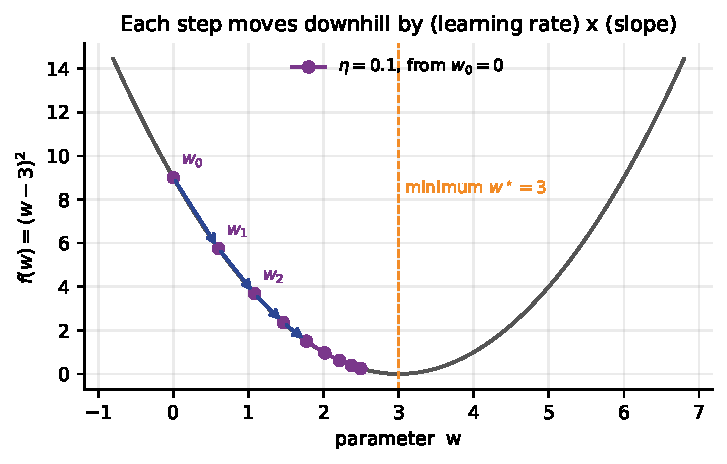
\includegraphics[width=0.72\textwidth]{gdsteps.pdf}
  \caption{Gradient descent on $f(w)=(w-3)^2$ from $w_0=0$ with $\eta=0.1$.
  The arrows mark the first four steps. Points bunch up near the minimum
  because the slope --- and therefore the step --- is shrinking.}
  \label{fig:gdsteps}
\end{figure}

\begin{keyidea}
On a quadratic, gradient descent multiplies the remaining error by a fixed
factor every iteration. Convergence is \textbf{geometric}: each step buys the
same \emph{percentage} improvement, not the same absolute improvement. That is
why loss curves look like a cliff followed by a long flat tail, and why the
last decimal place always costs the most.
\end{keyidea}

\subsection{Many parameters}

With $p$ parameters, $w$ is a vector and the derivative becomes the
\textbf{gradient} --- the vector of partial derivatives,
\[
  \nabla J(w) \;=\;
  \Big[\, \tfrac{\partial J}{\partial w_1},\;
          \tfrac{\partial J}{\partial w_2},\; \dots,\;
          \tfrac{\partial J}{\partial w_p} \,\Big]^\top .
\]

The gradient points in the direction of \emph{steepest increase} of $J$, so
$-\nabla J$ points in the direction of steepest decrease. The update is
unchanged in form:

\begin{equation}
  \label{eq:gd}
  w \;\leftarrow\; w \;-\; \eta \, \nabla J(w).
\end{equation}

For the mean squared error of a linear model,
$J(w) = \frac{1}{n}\sum_i (x_i^\top w - y_i)^2 = \frac{1}{n}\lVert Xw-y\rVert^2$,
the gradient is
\begin{equation}
  \label{eq:lsgrad}
  \nabla J(w) \;=\; \frac{2}{n}\, X^\top (Xw - y).
\end{equation}
That single line is the only calculus this lecture needs, and every code
example below is a direct transcription of it.

\begin{caution}[``Steepest descent'' is a local claim, not a global one]
$-\nabla J$ is the best direction \emph{for an infinitesimally small step}. It
is not the direction of the minimum. On a stretched bowl the two can be almost
perpendicular --- which is exactly the ravine problem that motivates momentum
in Section~\ref{sec:momentum}.
\end{caution}

% =========================================================================
\section{The learning rate}
\label{sec:lr}

Equation~\eqref{eq:contract} tells us everything about how $\eta$ behaves on a
quadratic. The error multiplier is $\lvert 1 - 2\eta\rvert$ for
$f(w) = (w-3)^2$, and in general $\lvert 1 - \eta f''\rvert$ where $f''$ is the
curvature. Four regimes follow immediately.

\begin{center}
\begin{tabular}{@{}llp{7.6cm}@{}}
\toprule
\textbf{Regime} & \textbf{Multiplier} & \textbf{Behaviour}\\
\midrule
$\eta$ too small     & just under $1$ & converges, but takes forever\\[3pt]
$\eta$ well chosen   & near $0$       & converges fast, monotonically\\[3pt]
$\eta$ too large     & between $-1$ and $0$ & converges, but overshoots and
  oscillates about the minimum\\[3pt]
$\eta$ past the limit & magnitude $> 1$ & \textbf{diverges}: each step is
  further out than the last\\
\bottomrule
\end{tabular}
\end{center}

Setting $\lvert 1 - \eta f''\rvert < 1$ gives the \textbf{stability threshold}

\begin{equation}
  \label{eq:stab}
  0 \;<\; \eta \;<\; \frac{2}{L},
  \qquad L = \text{the largest curvature of } J .
\end{equation}

For $f(w) = (w-3)^2$ we have $f'' = 2$, so the threshold is exactly
$\eta < 1$. And the multiplier is exactly zero when $\eta = 1/f'' = 0.5$ ---
gradient descent then lands on the minimum in a \emph{single step}, because for
a quadratic that step is Newton's method.

\begin{worked}[The four regimes, worked out]
Still $f(w) = (w-3)^2$, still $w_0 = 0$, twenty iterations.

\begin{center}
\begin{tabular}{@{}rrl@{}}
\toprule
$\eta$ & $\lvert 1-2\eta \rvert$ & prediction\\
\midrule
$0.10$ & $0.80$ & converges slowly, from below\\
$0.50$ & $0.00$ & \textbf{exact after one step}\\
$0.90$ & $0.80$ & converges at the same rate as $0.10$, but oscillating\\
$1.00$ & $1.00$ & never converges, never diverges: bounces $0 \to 6 \to 0$\\
$1.05$ & $1.10$ & diverges\\
\bottomrule
\end{tabular}
\end{center}

The pair $\eta = 0.1$ and $\eta = 0.9$ is the one to think about. Both give
$\lvert 1-2\eta\rvert = 0.8$, so both converge at \emph{exactly the same speed},
one creeping up from below and one flipping from side to side. A learning rate
nine times larger bought nothing at all.
\end{worked}

\begin{lstlisting}
for eta in [0.1, 0.5, 0.9, 1.0, 1.05]:
    w = 0.0
    for _ in range(20):
        w = w - eta*2.0*(w - 3.0)
    print("eta=%4.2f   |1-2*eta| = %.2f   w_20 = %12.4f" % (eta, abs(1-2*eta), w))
\end{lstlisting}
\begin{codeout}
eta=0.10   |1-2*eta| = 0.80   w_20 =       2.9654
eta=0.50   |1-2*eta| = 0.00   w_20 =       3.0000
eta=0.90   |1-2*eta| = 0.80   w_20 =       2.9654
eta=1.00   |1-2*eta| = 1.00   w_20 =       0.0000
eta=1.05   |1-2*eta| = 1.10   w_20 =     -17.1825
\end{codeout}

Every prediction is confirmed, including the two that look strange. At
$\eta = 0.9$ the answer after twenty steps is $2.9654$ --- the same to four
decimals as $\eta = 0.1$. At $\eta = 1.0$ the iterate is back exactly where it
started: $w$ alternates $0, 6, 0, 6, \dots$ forever, a perpetual-motion machine
that never makes progress. And a five per cent increase past the threshold,
from $1.00$ to $1.05$, turns that into $-17.18$ and falling.

\begin{figure}[htbp]
  \centering
  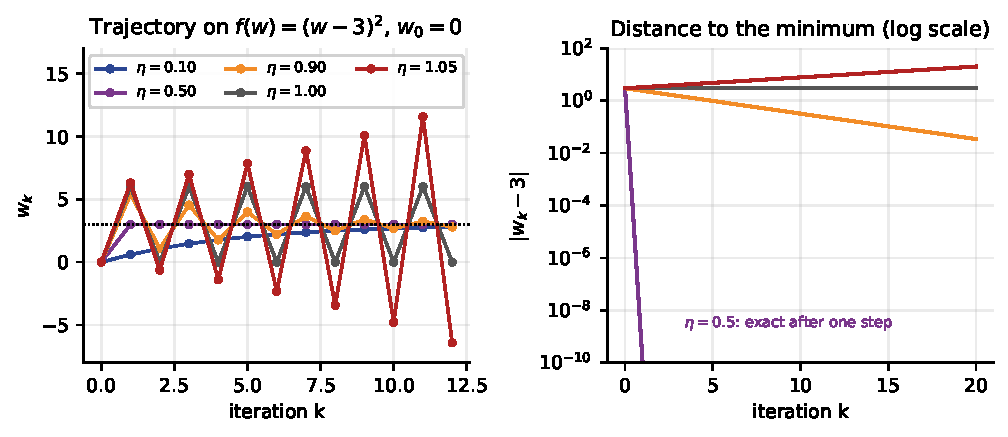
\includegraphics[width=0.94\textwidth]{lrgrid.pdf}
  \caption{The four regimes. Left: the iterates themselves. Right: distance to
  the minimum on a logarithmic scale, where geometric convergence is a straight
  line --- downwards for $\eta<1$, flat for $\eta=1$, upwards for $\eta=1.05$.
  The $\eta=0.5$ curve falls off the bottom of the axis after one step because
  the error is exactly zero.}
  \label{fig:lrgrid}
\end{figure}

\begin{keyidea}[The learning-rate cliff]
Convergence does not degrade gracefully as $\eta$ grows. Up to $2/L$ everything
works; past $2/L$ nothing does. There is no warning, and the transition is
sharp: in our example $\eta=1.00$ is neutral and $\eta=1.05$ is already
exploding. This is why a diverging loss is almost always a learning-rate
problem before it is anything else.
\end{keyidea}

\subsection{Reading a loss curve}

You will not usually know $L$, so you will diagnose $\eta$ from the loss curve
instead. The four regimes have four distinct signatures:

\begin{itemize}[leftmargin=*]
  \item \textbf{Still falling steeply when you stop} --- $\eta$ too small, or
    you stopped too early. Multiply $\eta$ by $3$, or train longer.
  \item \textbf{Falls fast, then flattens} --- healthy.
  \item \textbf{Falls, then bounces without settling} --- $\eta$ slightly too
    large, or the gradient noise floor of Section~\ref{sec:sgd}.
  \item \textbf{Rises, or becomes \texttt{nan}} --- past the threshold. Divide
    $\eta$ by $10$ and start again.
\end{itemize}

\begin{caution}[A good $\eta$ is a property of the data, not of the algorithm]
$L$ depends on how your features are scaled, so a learning rate that works on
standardised data can be catastrophic on raw data. This is the single strongest
practical argument for the scaling step you will meet in Unit IV, and it is
easy to measure --- see Section~\ref{sec:scaling}.
\end{caution}

% =========================================================================
\section{Batch gradient descent on real data}
\label{sec:batch}

Now the same algorithm on the bundled diabetes dataset. We standardise the ten
features and the target, which puts the loss at exactly $1.0$ when $w = 0$ and
makes every number below easy to interpret.

\begin{lstlisting}
from sklearn.datasets import load_diabetes

d = load_diabetes()
X = d.data
X = (X - X.mean(axis=0)) / X.std(axis=0)     # standardise the 10 features
y = d.target.astype(float)
y = (y - y.mean()) / y.std()                 # and the target
n, p = X.shape

H  = 2.0/n * (X.T @ X)                       # Hessian of the mean squared error
ev = np.linalg.eigvalsh(H)
print("examples n, features p   ", n, p)
print("largest curvature   L    %.4f" % ev.max())
print("smallest curvature       %.4f" % ev.min())
print("condition number         %.1f" % (ev.max()/ev.min()))
print("stability limit  2/L     %.4f" % (2/ev.max()))
\end{lstlisting}
\begin{codeout}
examples n, features p    442 10
largest curvature   L    8.0484
smallest curvature       0.0171
condition number         470.1
stability limit  2/L     0.2485
\end{codeout}

Three things are now known before we run anything. Any learning rate at or
above $0.2485$ will diverge. The curvature differs by a factor of $470$ between
the steepest and the shallowest direction --- remember that number, it is the
reason Section~\ref{sec:momentum} exists. And because the loss is quadratic in
$w$, all of this is exact, not a rule of thumb.

\begin{lstlisting}
def mse(X, y, w):
    r = X @ w - y
    return float(np.mean(r**2))

def grad(X, y, w):
    r = X @ w - y
    return 2.0/len(y) * (X.T @ r)

w = np.zeros(p)
print("epoch  0   MSE %.4f" % mse(X, y, w))
for epoch in range(1, 6):
    w = w - 0.005*grad(X, y, w)
    print("epoch %2d   MSE %.4f" % (epoch, mse(X, y, w)))
w_star = np.linalg.lstsq(X, y, rcond=None)[0]
print("least-squares optimum  MSE %.4f" % mse(X, y, w_star))
\end{lstlisting}
\begin{codeout}
epoch  0   MSE 1.0000
epoch  1   MSE 0.9713
epoch  2   MSE 0.9447
epoch  3   MSE 0.9199
epoch  4   MSE 0.8969
epoch  5   MSE 0.8754
least-squares optimum  MSE 0.4823
\end{codeout}

This is what \textbf{batch gradient descent} looks like: one update per pass
over the data, using the gradient computed from all $442$ examples. Five passes
have closed about a quarter of the gap between $1.0000$ and $0.4823$. It works,
and it is slow.

\begin{keyidea}[Vocabulary, fixed now so it stays fixed]
An \textbf{epoch} is one complete pass over the training set. An
\textbf{update} (or iteration, or step) is one application of
Equation~\eqref{eq:gd}. Batch gradient descent performs exactly one update per
epoch. The methods in the next two sections perform many, and that difference
is the entire content of Sections~\ref{sec:sgd} and~\ref{sec:mini}.
\end{keyidea}

\subsection{The cost of one update}

Computing $\nabla J$ from Equation~\eqref{eq:lsgrad} touches every row of $X$:
the cost is $O(np)$ per update. With $n = 442$ that is instant. With
$n = 10^8$ --- a modest industrial dataset --- a single step of batch gradient
descent means reading a hundred million rows off disk, and you would need
thousands of such steps.

That is the observation the rest of this lecture is built on.

% =========================================================================
\section{Stochastic gradient descent}
\label{sec:sgd}

\subsection{The structure we have been ignoring}

The cost is an \emph{average} over the training set:
\[
  J(w) \;=\; \frac{1}{n}\sum_{i=1}^{n} \ell_i(w),
  \qquad\text{so}\qquad
  \nabla J(w) \;=\; \frac{1}{n}\sum_{i=1}^{n} \nabla \ell_i(w) .
\]

Batch gradient descent computes all $n$ terms of that sum and then takes one
step. But if you want to estimate an average, you do not need every term ---
you need a sample. Pick one index $i$ uniformly at random. Then

\begin{equation}
  \label{eq:unbiased}
  \mathbb{E}_i\big[\nabla \ell_i(w)\big]
  \;=\; \sum_{i=1}^{n} \frac{1}{n}\, \nabla \ell_i(w)
  \;=\; \nabla J(w).
\end{equation}

The gradient of a single randomly chosen example is an \textbf{unbiased
estimate} of the full gradient. It is a very noisy estimate --- but it is
correct on average, and it costs $1/n$ as much.

\textbf{Stochastic gradient descent} (SGD) takes that estimate and steps with
it anyway:
\begin{equation}
  \label{eq:sgd}
  \text{pick } i \text{ at random}; \qquad
  w \;\leftarrow\; w - \eta\, \nabla \ell_i(w).
\end{equation}

In one pass over the data, SGD performs $n$ updates where batch gradient
descent performs one --- for the same total arithmetic.

\begin{keyidea}
Batch gradient descent takes one very good step per epoch. SGD takes $n$
mediocre steps per epoch. Because progress compounds and the errors partly
cancel, $n$ mediocre steps beat one good step by a wide margin, and the margin
grows with $n$.
\end{keyidea}

\subsection{By hand, on three points}

\begin{worked}[One epoch of SGD against one batch step]
Three examples, one feature, no intercept: predict $\hat y = wx$ with
\[
  x = (1,\, 2,\, 3), \qquad y = (2,\, 4,\, 7).
\]
The per-example loss is $\ell_i(w) = (w x_i - y_i)^2$, so
$\nabla \ell_i(w) = 2 x_i (w x_i - y_i)$. Start at $w = 0$ with $\eta = 0.05$.

\medskip
\textbf{One batch step.} The full gradient is the mean of the three:
\[
  \nabla J(0) = \tfrac{1}{3}\big[2(1)(0-2) + 2(2)(0-4) + 2(3)(0-7)\big]
              = \tfrac{1}{3}\big[-4 - 16 - 42\big] = -20.6667 .
\]
\[
  w \leftarrow 0 - 0.05 \times (-20.6667) = \mathbf{1.0333}.
\]

\medskip
\textbf{One epoch of SGD}, visiting the examples in order:
\begin{center}
\begin{tabular}{@{}clrr@{}}
\toprule
step & gradient at the current $w$ & value & new $w$\\
\midrule
$x=1$ & $2(1)(0 \cdot 1 - 2)$        & $-4.0000$  & $0.2000$\\
$x=2$ & $2(2)(0.2 \cdot 2 - 4)$      & $-14.4000$ & $0.9200$\\
$x=3$ & $2(3)(0.92 \cdot 3 - 7)$     & $-25.4400$ & $\mathbf{2.1920}$\\
\bottomrule
\end{tabular}
\end{center}

The exact least-squares answer is
$w^\star = \frac{\sum x_i y_i}{\sum x_i^2} = \frac{31}{14} = 2.2143$.

After the same amount of arithmetic --- three per-example gradients either way
--- batch gradient descent is at $1.0333$ and SGD is at $2.1920$, within one
per cent of the exact optimum.

Why? Because SGD's second gradient was evaluated at $w = 0.2$ rather than at
$w = 0$. It used information the batch method threw away by insisting on
finishing the sum first.
\end{worked}

\begin{lstlisting}
xs = np.array([1., 2., 3.])
ys = np.array([2., 4., 7.])
eta = 0.05

w = 0.0
g = np.mean(2*xs*(w*xs - ys))
print("one full-batch step:  gradient %+.4f  ->  w = %.4f" % (g, w - eta*g))

w = 0.0
for xi, yi in zip(xs, ys):
    gi = 2*xi*(w*xi - yi)
    w = w - eta*gi
    print("  SGD on x=%.0f:      gradient %+.4f  ->  w = %.4f" % (xi, gi, w))
print("least-squares optimum w* = %.4f" % (np.sum(xs*ys)/np.sum(xs*xs)))
\end{lstlisting}
\begin{codeout}
one full-batch step:  gradient -20.6667  ->  w = 1.0333
  SGD on x=1:      gradient -4.0000  ->  w = 0.2000
  SGD on x=2:      gradient -14.4000  ->  w = 0.9200
  SGD on x=3:      gradient -25.4400  ->  w = 2.1920
least-squares optimum w* = 2.2143
\end{codeout}

\begin{caution}[Shuffle every epoch]
The example above visited the points in a fixed order, which is fine for a
demonstration and wrong in practice. If your data is sorted by label --- and
data very often is --- fixed-order SGD spends the first half of every epoch
pulling the parameters towards one class and the second half pulling them back.
Draw a fresh permutation at the start of each epoch. Every implementation below
does.
\end{caution}

\subsection{The price: SGD never quite arrives}

Unbiased does not mean noiseless. Near the optimum the full gradient is nearly
zero, but the individual $\nabla \ell_i$ are not: they point in all directions
and cancel only on average. So SGD with a fixed step size does not converge to
$w^\star$. It converges to a \emph{cloud} around $w^\star$ whose size grows
with $\eta$ --- the \textbf{noise floor}.

The classical fix is to shrink the step size over time. The Robbins--Monro
conditions say a schedule $\eta_t$ guarantees convergence if
\[
  \sum_{t=1}^{\infty} \eta_t = \infty
  \qquad\text{and}\qquad
  \sum_{t=1}^{\infty} \eta_t^2 < \infty .
\]
The first condition says the steps must not shrink so fast that you stop before
arriving; the second says they must shrink fast enough to damp the noise.
$\eta_t = \eta_0/(1 + ct)$ satisfies both. Here is the effect, measured.

\begin{lstlisting}
def run_decay(eta0=0.02, epochs=30, seed=1, decay=True):
    rng = np.random.default_rng(seed); w = np.zeros(p); t = 0
    for _ in range(epochs):
        for i in rng.permutation(n):
            t += 1
            eta = eta0/(1 + 0.002*t) if decay else eta0
            w = w - eta*grad(X[i:i+1], y[i:i+1], w)
    return mse(X, y, w)

print("SGD (B=1, 30 epochs), constant step 0.02   MSE %.4f" % run_decay(decay=False))
print("SGD (B=1, 30 epochs), decayed step         MSE %.4f" % run_decay(decay=True))
print("least-squares optimum                      MSE %.4f" % mse(X, y, w_star))
\end{lstlisting}
\begin{codeout}
SGD (B=1, 30 epochs), constant step 0.02   MSE 0.5395
SGD (B=1, 30 epochs), decayed step         MSE 0.4834
least-squares optimum                      MSE 0.4823
\end{codeout}

With a constant step the run stalls at $0.5395$ and stays there --- it is not
converging slowly, it is orbiting. Decaying the step closes almost the entire
remaining gap, reaching $0.4834$ against an optimum of $0.4823$.

\begin{caution}[Two different things look the same on a loss curve]
A loss that bounces without settling can mean $\eta$ is above the stability
threshold, \emph{or} that you have reached the SGD noise floor. They need
opposite responses --- reduce $\eta$ in both cases, but in the first the
training is broken and in the second it is finished. Distinguish them by
evaluating the loss on the \emph{whole} training set rather than on the current
mini-batch: a true divergence rises, a noise floor is flat with jitter.
\end{caution}

% =========================================================================
\section{Mini-batch gradient descent}
\label{sec:mini}

Batch gradient descent uses $n$ examples per update; SGD uses $1$. Nothing
forces those to be the only options. \textbf{Mini-batch gradient descent} uses
$B$ examples, with $1 \le B \le n$:

\begin{equation}
  \label{eq:mb}
  w \;\leftarrow\; w \;-\; \eta \, \frac{1}{B}\sum_{i \in \mathcal{B}}
    \nabla \ell_i(w),
  \qquad \mathcal{B} \text{ a random subset of size } B .
\end{equation}

Batch and stochastic gradient descent are the two endpoints, $B = n$ and
$B = 1$. In practice the answer is always somewhere in between, and this
section is about why.

\subsection{How the noise depends on $B$}

Averaging $B$ independent unbiased estimates divides the variance by $B$, so
the \emph{standard deviation} of the mini-batch gradient falls like
$1/\sqrt{B}$. That is the central trade-off in one line, and we can measure it
exactly.

\begin{lstlisting}
rng = np.random.default_rng(0)
w0 = np.zeros(p)
g_full = grad(X, y, w0)
print("|| full gradient ||  %.4f" % np.linalg.norm(g_full))
for B in [1, 2, 4, 8, 16, 32, 64, 128, 256]:
    sq = []
    for _ in range(3000):
        idx = rng.choice(n, size=B, replace=False)
        sq.append(np.sum((grad(X[idx], y[idx], w0) - g_full)**2))
    print("B=%4d   RMS ||g_B - g|| = %.4f" % (B, np.sqrt(np.mean(sq))))
\end{lstlisting}
\begin{codeout}
|| full gradient ||  2.4157
B=   1   RMS ||g_B - g|| = 6.3234
B=   2   RMS ||g_B - g|| = 4.4099
B=   4   RMS ||g_B - g|| = 3.1309
B=   8   RMS ||g_B - g|| = 2.1805
B=  16   RMS ||g_B - g|| = 1.5199
B=  32   RMS ||g_B - g|| = 1.0641
B=  64   RMS ||g_B - g|| = 0.7152
B= 128   RMS ||g_B - g|| = 0.4617
B= 256   RMS ||g_B - g|| = 0.2507
\end{codeout}

Read the first two lines together and be slightly alarmed: the full gradient
has length $2.4157$, and a single-example gradient is typically wrong by
$6.3234$ --- an error more than \emph{twice the size of the thing being
estimated}. A single stochastic step frequently points uphill. It still works,
because the errors cancel over many steps.

Now read down the column. Each doubling of $B$ multiplies the error by about
$1/\sqrt{2} \approx 0.707$: $6.32 \to 4.41 \to 3.13 \to 2.18 \to 1.52$. Going
from $B=1$ to $B=32$ costs $32$ times more arithmetic per update and buys a
factor of only $6.32/1.06 = 5.9$ --- almost exactly $\sqrt{32} = 5.66$.

\begin{figure}[htbp]
  \centering
  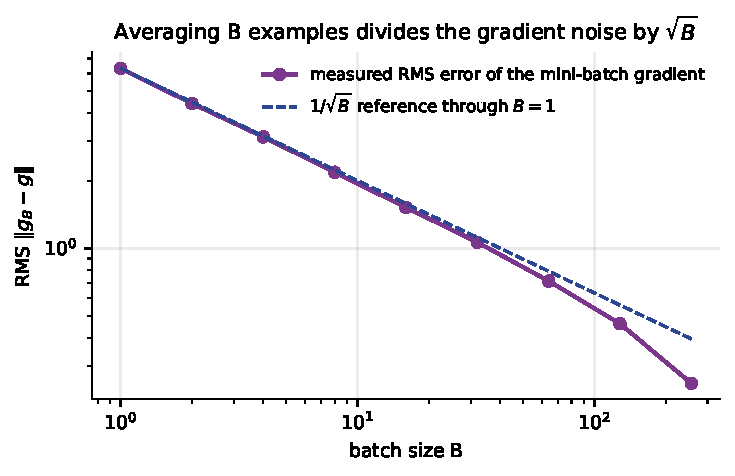
\includegraphics[width=0.70\textwidth]{gradnoise.pdf}
  \caption{Measured RMS error of the mini-batch gradient against batch size,
  log--log, with a $1/\sqrt{B}$ reference line. The measured curve falls below
  the reference at large $B$ because we sample \emph{without} replacement, so a
  batch of $256$ out of $442$ already contains most of the data; at $B=n$ the
  error is exactly zero.}
  \label{fig:gradnoise}
\end{figure}

\begin{keyidea}[The diminishing return that decides everything]
Gradient quality improves as $\sqrt{B}$ while cost grows as $B$. Doubling the
batch size therefore buys you $41\%$ less noise for $100\%$ more work. Large
batches are a bad deal for accuracy --- which is why nobody uses $B=n$.
\end{keyidea}

\subsection{Progress per epoch}

If small batches give better value per unit of arithmetic, why not $B=1$? Run
all three for thirty epochs at the same learning rate.

\begin{lstlisting}
def run(B, epochs=30, eta=0.005, seed=1):
    rng = np.random.default_rng(seed)
    w = np.zeros(p)
    hist = [mse(X, y, w)]
    for _ in range(epochs):
        order = rng.permutation(n) if B < n else np.arange(n)
        for s in range(0, n, B):
            idx = order[s:s+B]
            w = w - eta*grad(X[idx], y[idx], w)
        hist.append(mse(X, y, w))
    return np.array(hist)

h_batch, h_mini, h_sgd = run(n), run(32), run(1)
print("                updates/epoch   after 1 epoch   after 30 epochs")
print("batch  B=442              1          %.4f            %.4f" % (h_batch[1], h_batch[30]))
print("mini   B= 32             14          %.4f            %.4f" % (h_mini[1],  h_mini[30]))
print("SGD    B=  1            442          %.4f            %.4f" % (h_sgd[1],   h_sgd[30]))
print("least-squares optimum                                  %.4f" % mse(X, y, w_star))
\end{lstlisting}
\begin{codeout}
                updates/epoch   after 1 epoch   after 30 epochs
batch  B=442              1          0.9713            0.6219
mini   B= 32             14          0.7393            0.4860
SGD    B=  1            442          0.5268            0.4859
least-squares optimum                                  0.4823
\end{codeout}

Every one of those rows used the same number of per-example gradient
evaluations. After thirty epochs batch gradient descent has reached $0.6219$,
still a long way from $0.4823$, while both stochastic methods have essentially
finished. And after a \emph{single} epoch SGD is already at $0.5268$ --- better
than batch gradient descent manages in thirty.

That comparison deserves a number of its own.

\begin{lstlisting}
target = h_sgd[1]
h_long = run(n, epochs=3000)
print("SGD reaches MSE %.4f after a single epoch." % target)
print("Full-batch GD needs %d epochs to reach the same MSE." % np.argmax(h_long <= target))
\end{lstlisting}
\begin{codeout}
SGD reaches MSE 0.5268 after a single epoch.
Full-batch GD needs 80 epochs to reach the same MSE.
\end{codeout}

\textbf{Eighty passes over the data against one.} Both spend the same
arithmetic per pass. The whole of that factor comes from SGD updating its
parameters $442$ times per pass instead of once.

\begin{figure}[htbp]
  \centering
  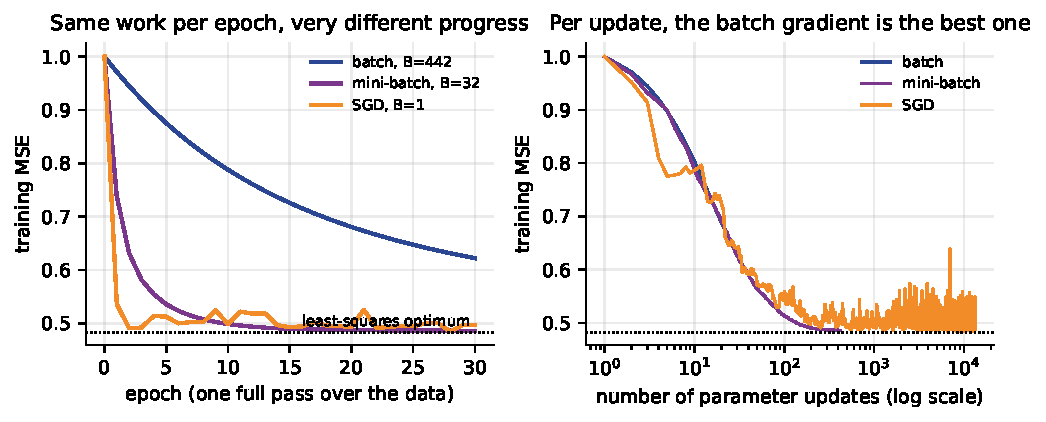
\includegraphics[width=0.94\textwidth]{epochs.pdf}
  \caption{Left: training MSE per epoch --- equal work along the horizontal
  axis, and the small batches win overwhelmingly. Right: the same runs plotted
  against the number of parameter updates, where the ordering reverses. Per
  update the batch gradient is the best one; per unit of work it is by far the
  worst.}
  \label{fig:epochs}
\end{figure}

The two panels of Figure~\ref{fig:epochs} contradict each other, and both are
true. Per \emph{update}, more data is better --- the blue curve on the right
descends fastest. Per unit of \emph{work}, more data is worse --- the same
curve on the left descends slowest. Optimisation is judged by the second
criterion, because work is what you pay for. The right-hand panel also shows
the noise floor plainly: past about a hundred updates the SGD curve stops
descending and becomes a band of jitter around $0.49$.

\subsection{So why not $B=1$?}

Because arithmetic operations are not the same thing as time. A mini-batch
gradient is one matrix--vector product; a hundred single-example gradients are
a hundred tiny operations, each carrying the full overhead of a Python-level
loop, a memory allocation and a kernel launch.

\begin{lstlisting}
import time
for B in (1, 32, 442):
    best = float("inf")
    for _ in range(25):
        w = np.zeros(p)
        t0 = time.perf_counter()
        for s in range(0, n, B):
            w = w - 0.005*grad(X[s:s+B], y[s:s+B], w)
        best = min(best, time.perf_counter() - t0)
    print("B=%4d   %3d updates/epoch   %7.3f ms per epoch" % (B, -(-n//B), best*1000))
\end{lstlisting}
\begin{codeout}
B=   1   442 updates/epoch     1.224 ms per epoch
B=  32    14 updates/epoch     0.040 ms per epoch
B= 442     1 updates/epoch     0.005 ms per epoch
\end{codeout}

Identical arithmetic; \textbf{$31$ times} the wall-clock cost for $B=1$ against
$B=32$ on this machine. And $B=32$ reached MSE $0.4860$ after thirty epochs
against SGD's $0.4859$ --- statistically the same answer, thirty-one times
faster.

\begin{caution}[These timings are machine-dependent]
The ratio, not the absolute times, is the point. On a GPU the effect is far
larger: a device with thousands of cores is almost entirely idle processing one
example at a time, and batch sizes of $256$ or $1024$ can cost no more
wall-clock time per update than a batch of $32$.
\end{caution}

\begin{figure}[htbp]
  \centering
  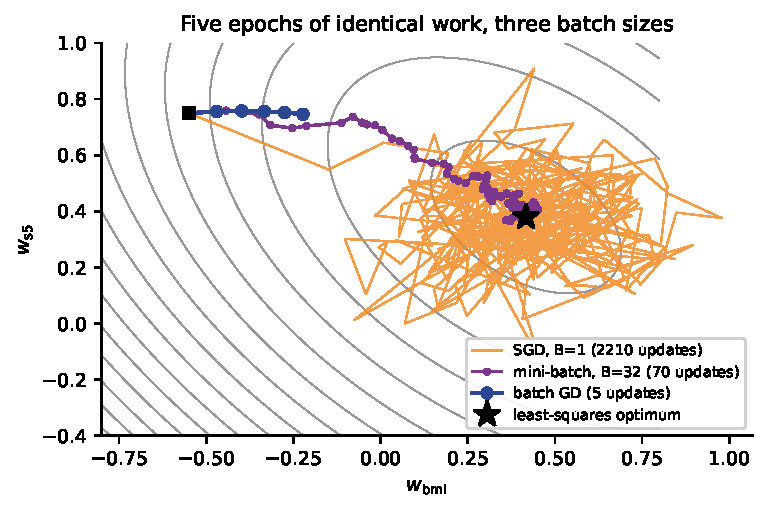
\includegraphics[width=0.76\textwidth]{sgdpath.pdf}
  \caption{Five epochs of identical work on a two-parameter version of the
  problem (features \texttt{bmi} and \texttt{s5}). Batch gradient descent
  manages five updates and barely leaves the start. Mini-batch takes a fairly
  direct path in $70$ updates. SGD's $2210$ updates arrive quickly and then
  rattle around the optimum without settling --- the noise floor, seen from
  above.}
  \label{fig:sgdpath}
\end{figure}

\subsection{The summary table}

\begin{center}
\begin{tabular}{@{}lccccc@{}}
\toprule
& \textbf{$B$} & \textbf{updates/epoch} & \textbf{gradient noise}
& \textbf{cost/update} & \textbf{vectorises}\\
\midrule
Batch      & $n$   & $1$   & none          & $O(np)$ & yes\\
Mini-batch & $32$--$512$ & $n/B$ & moderate & $O(Bp)$ & yes\\
Stochastic & $1$   & $n$   & large         & $O(p)$  & no\\
\bottomrule
\end{tabular}
\end{center}

\begin{keyidea}[Why mini-batch wins]
Mini-batch gradient descent is not a compromise that is slightly worse than
both extremes. It is strictly better than both. It keeps almost all of SGD's
update frequency --- $14$ updates per epoch instead of $1$ was enough to reach
the optimum here --- while recovering the vectorised arithmetic that makes
hardware fast, and cutting the gradient noise by $\sqrt{B}$ into the bargain.
It is the default in every deep-learning framework for these reasons and no
others.
\end{keyidea}

\begin{caution}[Terminology in the wild]
Almost everything called ``SGD'' in a paper, a library or a job advert is
mini-batch gradient descent. \texttt{torch.optim.SGD} takes whatever batch size
your data loader produces. Genuine one-example-at-a-time SGD is rare outside
online-learning settings. When someone says SGD, assume $B > 1$ unless they say
otherwise.
\end{caution}

\subsection{Choosing $B$ in practice}

\begin{itemize}[leftmargin=*]
  \item Start at $B = 32$: the commonest default, and rarely a bad one.
  \item Use powers of two --- memory alignment and GPU kernels are built around
    them, and $B=32$ and $B=33$ can differ measurably in speed.
  \item The binding constraint is usually memory, not statistics.
  \item If you increase $B$ you may increase $\eta$, because the gradient is
    less noisy; a common rule of thumb is to scale $\eta$ linearly with $B$.
  \item Tune $\eta$ before $B$. The learning rate matters far more.
\end{itemize}

\begin{tryit}
Re-run the \texttt{run()} function above with $B = 4, 8, 64, 128$ and plot MSE
after five epochs against $B$. You should find a broad flat region rather than
a sharp optimum --- which is exactly why $B=32$ is a safe default and why it is
not worth much tuning effort.
\end{tryit}

\newpage
% =========================================================================
\section{Momentum}
\label{sec:momentum}

\subsection{The problem momentum solves}

Recall the number we measured in Section~\ref{sec:batch}: the curvature of our
loss differs by a factor of $470$ between the steepest and the shallowest
direction. Such a loss surface is a \textbf{ravine} --- a long, narrow valley
with steep walls and a gently sloping floor.

Gradient descent handles a ravine badly, and Equation~\eqref{eq:stab} says
exactly why. The learning rate must satisfy $\eta < 2/L$ where $L$ is the
\emph{largest} curvature, so $\eta$ is dictated by the steep walls. But the
progress that matters is along the floor, where the curvature is $L/470$. The
result: the iterates bounce from wall to wall while creeping along the valley.
The step size that keeps the crossing direction stable is $470$ times too small
for the direction we actually care about.

\begin{keyidea}
In a ravine, gradient descent is limited by the direction you do not want to
travel in. Momentum exists to break that coupling.
\end{keyidea}

\subsection{The heavy ball}

Think of a ball rolling down the valley rather than a hiker taking independent
steps. The ball accumulates velocity. Along the floor, where the slope points
the same way every step, velocity builds up and the ball accelerates. Across
the valley, where the slope reverses every step, the contributions cancel and
the oscillation is damped.

Written out, with a \textbf{velocity} vector $v$ and a momentum coefficient
$\beta \in [0,1)$:

\begin{equation}
  \label{eq:mom}
  v \;\leftarrow\; \beta\, v \;+\; \nabla J(w),
  \qquad
  w \;\leftarrow\; w \;-\; \eta\, v .
\end{equation}

Setting $\beta = 0$ recovers plain gradient descent exactly. This is Polyak's
heavy-ball method, and it is the form used by \texttt{torch.optim.SGD} and by
\emph{Dive into Deep Learning} \S12.6.

\subsection{Momentum is an exponentially weighted average}

Unroll the recursion for $v$, starting from $v_0 = 0$:
\[
  v_t = \beta v_{t-1} + g_t
      = g_t + \beta g_{t-1} + \beta^2 g_{t-2} + \cdots
      = \sum_{j=0}^{t-1} \beta^{\,j} g_{t-j}.
\]

The velocity is a weighted sum of \emph{all} past gradients, with weights
decaying geometrically. Recent gradients dominate; a gradient from $20$ steps
ago carries weight $0.9^{20} = 0.12$.

The total weight is the geometric series
\[
  \sum_{j=0}^{\infty} \beta^{\,j} = \frac{1}{1-\beta}.
\]

That gives the number worth memorising. If the gradient is roughly constant
over many steps --- which is precisely the situation along the valley floor ---
then $v$ settles at about $g/(1-\beta)$ and the effective step becomes

\begin{equation}
  \label{eq:effstep}
  \eta_{\text{eff}} \;\approx\; \frac{\eta}{1-\beta}.
\end{equation}

With $\beta = 0.9$ that is $10\eta$; with $\beta = 0.99$ it is $100\eta$.
Momentum is a $10\times$ speed-up in consistent directions, obtained without
raising $\eta$ in the inconsistent ones.

\begin{worked}[Four steps of momentum, on paper]
Back to $f(w) = (w-3)^2$, $\eta = 0.1$, now with $\beta = 0.9$. Start
$w_0 = 0$, $v_0 = 0$, and recall $g = 2(w-3)$.

\begin{center}
\begin{tabular}{@{}rrrl@{}}
\toprule
$k$ & $g_k$ & $v_k = 0.9 v_{k-1} + g_k$ & $w_k = w_{k-1} - 0.1 v_k$\\
\midrule
1 & $-6.0000$ & $0 - 6.0000 = -6.0000$              & $0 + 0.6000 = 0.6000$\\
2 & $-4.8000$ & $-5.4000 - 4.8000 = -10.2000$       & $0.6 + 1.0200 = 1.6200$\\
3 & $-2.7600$ & $-9.1800 - 2.7600 = -11.9400$       & $1.62 + 1.1940 = 2.8140$\\
4 & $-0.3720$ & $-10.7460 - 0.3720 = -11.1180$      & $2.814 + 1.1118 = \mathbf{3.9258}$\\
\bottomrule
\end{tabular}
\end{center}

Compare with plain gradient descent, which was at $1.7712$ after four steps.
Momentum is at $3.9258$ --- it has already gone \emph{past} the minimum at $3$.

Look at row 4 to see how. The gradient there is nearly zero ($-0.372$, because
$w$ is close to $3$), yet the velocity is still $-11.12$, carrying nine tenths
of everything accumulated earlier. The ball arrives at the bottom of the bowl
travelling fast and rolls up the far side.
\end{worked}

\begin{lstlisting}
eta, beta = 0.1, 0.9
w, v = 0.0, 0.0
for k in range(1, 5):
    g = 2.0*(w - 3.0)
    v = beta*v + g
    w = w - eta*v
    print("k=%d   g=%+8.4f   v=%+9.4f   w=%.4f" % (k, g, v, w))
\end{lstlisting}
\begin{codeout}
k=1   g= -6.0000   v=  -6.0000   w=0.6000
k=2   g= -4.8000   v= -10.2000   w=1.6200
k=3   g= -2.7600   v= -11.9400   w=2.8140
k=4   g= -0.3720   v= -11.1180   w=3.9258
\end{codeout}

\subsection{Yes, momentum overshoots}

Overshooting is not a bug to be tuned away; it is inherent to the method, and
whether it is worth paying for depends entirely on the shape of the problem.
Here is the full picture on the same one-dimensional quadratic.

\begin{lstlisting}
for beta in (0.0, 0.5, 0.9):
    w, v, hit, top = 0.0, 0.0, None, 0.0
    for k in range(1, 201):
        v = beta*v + 2.0*(w - 3.0)
        w = w - 0.1*v
        top = max(top, w)
        if hit is None and abs(w - 3.0) < 1e-3:
            hit = k
    print("beta=%.1f   first k with |w-3|<1e-3: %3d   highest w reached: %.4f"
          % (beta, hit, top))
\end{lstlisting}
\begin{codeout}
beta=0.0   first k with |w-3|<1e-3:  36   highest w reached: 3.0000
beta=0.5   first k with |w-3|<1e-3:  20   highest w reached: 3.2092
beta=0.9   first k with |w-3|<1e-3:  92   highest w reached: 5.1269
\end{codeout}

Three different answers, and the middle one is the interesting one.

\begin{itemize}[leftmargin=*]
  \item $\beta = 0$: $36$ steps, never overshoots. Plain gradient descent
    approaches monotonically from below.
  \item $\beta = 0.5$: $20$ steps, overshoots to $3.2092$. Nearly twice as
    fast, at the cost of a small excursion past the target.
  \item $\beta = 0.9$: $92$ steps, overshoots to $5.1269$ --- it travels past
    the minimum at $3$ almost as far as it started from it. Two and a half
    times \emph{slower} than plain gradient descent.
\end{itemize}

\begin{figure}[htbp]
  \centering
  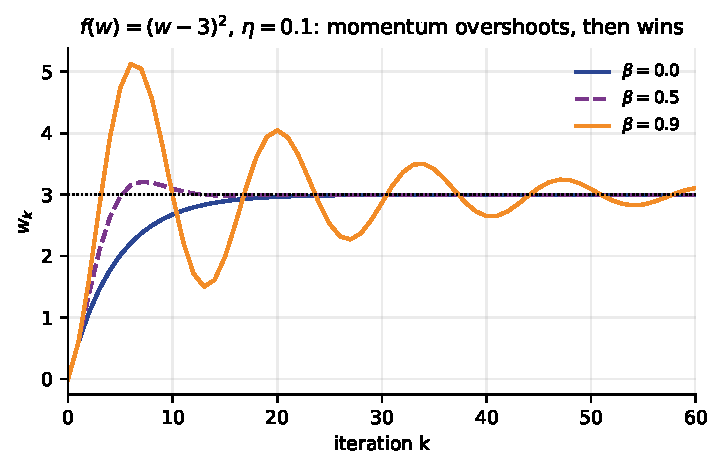
\includegraphics[width=0.72\textwidth]{momentum1d.pdf}
  \caption{Momentum on $f(w)=(w-3)^2$ with $\eta = 0.1$. Plain gradient descent
  (blue) climbs monotonically to $3$. $\beta=0.5$ (purple) gets there faster
  with a small overshoot. $\beta=0.9$ (orange) sails up to $5.13$ and spends
  the next eighty iterations ringing down.}
  \label{fig:momentum1d}
\end{figure}

\begin{caution}[Momentum does not help on a well-conditioned problem]
A one-dimensional quadratic has condition number $1$: there is no ravine, no
direction whose oscillation needs damping, and nothing for the accumulated
velocity to accelerate along. All momentum can do is overshoot. Setting
$\beta = 0.9$ here made the optimiser \textbf{two and a half times slower}.

Momentum is not a free improvement you sprinkle on. It is a targeted remedy for
badly conditioned problems --- which happens to describe almost every real
model, but not this one.
\end{caution}

\subsection{Now put it in a ravine}

Here is a quadratic built so we know its condition number exactly:
\[
  f(w) = 0.01\,w_1^2 + 2\,w_2^2,
  \qquad \nabla f(w) = (0.02\,w_1,\; 4\,w_2),
  \qquad \kappa = \frac{4}{0.02} = 200 .
\]
The stability ceiling for plain gradient descent is $2/L = 2/4 = 0.5$. We use
$\eta = 0.475$, which is $95\%$ of it --- as aggressive as plain gradient
descent is allowed to be.

\begin{lstlisting}
A = np.array([0.02, 4.0])            # Hessian diagonal: kappa = 200

def run_ravine(eta, beta, iters=1600):
    w = np.array([9.0, 1.0]); v = np.zeros(2)
    for k in range(1, iters+1):
        v = beta*v + A*w
        w = w - eta*v
        if not np.all(np.isfinite(w)) or np.linalg.norm(w) > 1e8:
            return "diverged at k=%d" % k
        if np.linalg.norm(w) < 1e-3:
            return k
    return "not reached in %d" % iters

print("plain-GD ceiling      2/L          = %.3f" % (2/A.max()))
print("momentum ceiling  2(1+beta)/L      = %.3f   (beta=0.9)" % (2*1.9/A.max()))
for beta in (0.0, 0.5, 0.9):
    print("eta=0.475  beta=%.1f   iterations to ||w||<1e-3:  %s"
          % (beta, run_ravine(0.475, beta)))
for beta in (0.0, 0.9):
    print("eta=0.900  beta=%.1f   iterations to ||w||<1e-3:  %s"
          % (beta, run_ravine(0.900, beta)))
\end{lstlisting}
\begin{codeout}
plain-GD ceiling      2/L          = 0.500
momentum ceiling  2(1+beta)/L      = 0.950   (beta=0.9)
eta=0.475  beta=0.0   iterations to ||w||<1e-3:  954
eta=0.475  beta=0.5   iterations to ||w||<1e-3:  467
eta=0.475  beta=0.9   iterations to ||w||<1e-3:  135
eta=0.900  beta=0.0   iterations to ||w||<1e-3:  diverged at k=20
eta=0.900  beta=0.9   iterations to ||w||<1e-3:  161
\end{codeout}

Same learning rate, same starting point, same problem. Plain gradient descent
needs $954$ iterations; $\beta = 0.9$ needs $135$. That is a
\textbf{$7.1\times$ speed-up} from one extra line of code and one extra vector
of state.

The last two lines make a second, independent point. At $\eta = 0.9$ plain
gradient descent blows up within twenty iterations, because $0.9$ is well past
its ceiling of $0.5$. Momentum survives, because its stability ceiling is
\begin{equation}
  \label{eq:momstab}
  \eta \;<\; \frac{2(1+\beta)}{L},
\end{equation}
which for $\beta = 0.9$ is $0.95$. Momentum does not merely use the permitted
learning rates better --- it enlarges the set of permitted learning rates by a
factor of $1+\beta$.

\begin{figure}[htbp]
  \centering
  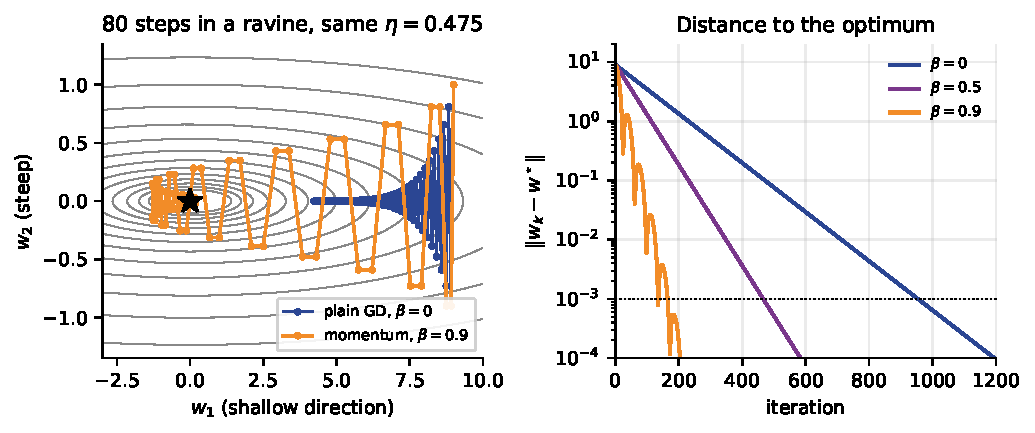
\includegraphics[width=0.94\textwidth]{ravine.pdf}
  \caption{Left: eighty steps in the ravine at $\eta = 0.475$. Plain gradient
  descent (blue) oscillates across the narrow direction and creeps along the
  floor, still near $w_1 = 7$ after eighty steps. Momentum (orange) oscillates
  too --- more violently, in fact --- but travels the length of the valley and
  reaches the optimum. Right: distance to the optimum on a log scale, where the
  slope of each line is the convergence rate.}
  \label{fig:ravine}
\end{figure}

Figure~\ref{fig:ravine} is worth a slow look, because the left panel does not
show what students usually expect. Momentum's path is \emph{messier} than
plain gradient descent's, not smoother. What it is not, is stuck. The lesson is
that momentum trades cross-valley tidiness for along-valley speed, and in a
ravine that is a trade you always want.

\subsection{The same thing on the real dataset}

The diabetes least-squares problem had condition number $470$ --- worse than
our synthetic ravine. Momentum should therefore help more, and it does.

\begin{lstlisting}
eta = 0.95*2/ev.max()
for beta in (0.0, 0.9):
    w, v = np.zeros(p), np.zeros(p)
    for k in range(1, 20001):
        v = beta*v + grad(X, y, w)
        w = w - eta*v
        if np.linalg.norm(w - w_star) < 1e-3:
            break
    print("beta=%.1f   eta=%.4f   full-batch iterations to the optimum: %5d"
          % (beta, eta, k))
\end{lstlisting}
\begin{codeout}
beta=0.0   eta=0.2361   full-batch iterations to the optimum:  1605
beta=0.9   eta=0.2361   full-batch iterations to the optimum:   128
\end{codeout}

$1605$ iterations down to $128$: a $12.5\times$ speed-up on real data, at the
same learning rate, from adding momentum. Notice that the speed-up ($12.5$) is
larger than the one on the synthetic ravine ($7.1$), and that the condition
number is larger too ($470$ against $200$). That is the general pattern: the
worse the conditioning, the more momentum is worth.

\subsection{Momentum with mini-batches}

In practice momentum is combined with mini-batch gradient descent, not with
full-batch. The update is identical --- substitute the mini-batch gradient for
$\nabla J$ in Equation~\eqref{eq:mom} --- and it now does two jobs at once:
it accelerates along consistent directions \emph{and} it averages away
sampling noise, since the exponentially weighted average of $1/(1-\beta) = 10$
recent mini-batch gradients is itself a lower-variance estimate.

\begin{lstlisting}
def run_mom(B, beta, eta, epochs=5, seed=1):
    rng = np.random.default_rng(seed)
    w, v = np.zeros(p), np.zeros(p)
    for _ in range(epochs):
        order = rng.permutation(n) if B < n else np.arange(n)
        for s in range(0, n, B):
            idx = order[s:s+B]
            v = beta*v + grad(X[idx], y[idx], w)
            w = w - eta*v
    return mse(X, y, w)

print("mini-batch B=32, eta=0.005, 5 epochs")
for beta in (0.0, 0.9, 0.99):
    print("   beta=%.2f   MSE %.4f" % (beta, run_mom(32, beta, 0.005)))
print("least-squares optimum   MSE %.4f" % mse(X, y, w_star))
\end{lstlisting}
\begin{codeout}
mini-batch B=32, eta=0.005, 5 epochs
   beta=0.00   MSE 0.5358
   beta=0.90   MSE 0.4870
   beta=0.99   MSE 0.5674
least-squares optimum   MSE 0.4823
\end{codeout}

Read the three rows carefully. Going from $\beta = 0$ to $\beta = 0.9$ moves
the five-epoch result from $0.5358$ to $0.4870$ --- most of the remaining gap
to the optimum, closed by one line. Going on to $\beta = 0.99$ makes things
\emph{worse} than no momentum at all, at $0.5674$: with an effective learning
rate of $100\eta$ the run is now overshooting badly.

\begin{caution}[When you raise $\beta$, lower $\eta$]
Equation~\eqref{eq:effstep} says the effective step is $\eta/(1-\beta)$. Moving
$\beta$ from $0.9$ to $0.99$ multiplies it by ten. If you change $\beta$ and
keep $\eta$, you have changed your learning rate by an order of magnitude
without meaning to, and the run above shows what that costs. As a rule of
thumb, scale $\eta$ by $(1-\beta_{\text{new}})/(1-\beta_{\text{old}})$.
\end{caution}

\begin{caution}[Two conventions, and they differ by a factor of $1-\beta$]
Some references and libraries write the velocity update as
\[
  v \leftarrow \beta v + (1-\beta)\, g
\]
instead of Equation~\eqref{eq:mom}. This is a true running average, so $v$ has
the same magnitude as $g$ rather than roughly $1/(1-\beta)$ times it. Andrew
Ng's course and the Adam paper use this form; PyTorch and \emph{Dive into Deep
Learning} use ours.

Both are correct, and they produce identical trajectories provided $\eta$ is
scaled by $1/(1-\beta)$ to match. Move code between them without rescaling and
your learning rate silently changes by a factor of ten. Always check which
convention a formula is written in before copying a value of $\eta$ out of it.
\end{caution}

\subsection{Choosing $\beta$}

\begin{itemize}[leftmargin=*]
  \item $\beta = 0.9$ is the default, and it is a good one. It corresponds to
    averaging roughly the last ten gradients.
  \item $\beta = 0.99$ averages the last hundred. Use it only on very noisy
    problems, and reduce $\eta$ tenfold when you do.
  \item $\beta = 0$ is not silly on a well-conditioned problem, as
    Section~\ref{sec:momentum} demonstrated.
  \item $\beta$ matters far less than $\eta$. Tune the learning rate first,
    then try $0.9$, and stop.
\end{itemize}

\begin{keyidea}[Momentum in one sentence]
Momentum replaces the current gradient with an exponentially weighted average
of recent gradients, which cancels the components that keep changing sign and
amplifies the components that do not --- turning a $954$-iteration crawl along
a ravine into a $135$-iteration run.
\end{keyidea}

Momentum treats every coordinate identically: one $\eta$, one $\beta$, applied
to the whole vector. L4 asks what happens when each coordinate gets its own
step size, adapted from the gradients that coordinate has seen --- Adagrad,
RMSprop and Adam.

% =========================================================================
\section{Putting it together}
\label{sec:practice}

\subsection{Feature scaling is an optimisation decision}
\label{sec:scaling}

Section~\ref{sec:lr} claimed that the usable learning rate is a property of
your data. Here is the measurement. We take the diabetes features and multiply
one of them by $1000$ --- an entirely realistic accident, the difference
between recording a quantity in kilometres and in metres.

\begin{lstlisting}
Xbad = load_diabetes().data.copy()
Xbad[:, 0] *= 1000.0                       # one feature on a wildly different scale
Xbad = Xbad - Xbad.mean(axis=0)
evb = np.linalg.eigvalsh(2.0/n * (Xbad.T @ Xbad))
print("condition number, standardised        %10.1f" % (ev.max()/ev.min()))
print("condition number, one feature x1000   %10.3e" % (evb.max()/evb.min()))
print("stability limit 2/L, standardised     %10.4f" % (2/ev.max()))
print("stability limit 2/L, unscaled         %10.3e" % (2/evb.max()))
\end{lstlisting}
\begin{codeout}
condition number, standardised             470.1
condition number, one feature x1000   1.168e+08
stability limit 2/L, standardised         0.2485
stability limit 2/L, unscaled          4.420e-04
\end{codeout}

The condition number rises from $470$ to $1.2 \times 10^8$, and the largest
usable learning rate falls by a factor of $560$. Since the number of iterations
grows with the condition number, this single unnoticed unit change turns a
problem that gradient descent solves in a few hundred iterations into one it
cannot solve at all in any reasonable time.

\begin{keyidea}
Standardising your features is not cosmetic and it is not only about
interpretability. It is the cheapest possible improvement to the conditioning
of your optimisation problem, and on gradient-based methods it is often the
difference between converging and not.
\end{keyidea}

\subsection{A recipe}

\begin{enumerate}[leftmargin=*]
  \item \textbf{Standardise the features.} Always, before anything else.
  \item \textbf{Choose $B = 32$} (or the largest power of two that fits
    comfortably in memory).
  \item \textbf{Find $\eta$ by bisection on a log scale.} Try
    $10^{-1}, 10^{-2}, 10^{-3}$ for a few epochs each. Take the largest that
    does not diverge, then back off by a factor of three.
  \item \textbf{Add momentum, $\beta = 0.9$.} If you had already tuned $\eta$
    without momentum, divide it by ten first.
  \item \textbf{Watch the loss curve} and match it against the four signatures
    in Section~\ref{sec:lr}.
  \item \textbf{Decay $\eta$ towards the end} if the curve flattens into a
    noisy band above where you expect it to finish.
\end{enumerate}

\subsection{What scikit-learn gives you}

\begin{sloppypar}
\texttt{SGDRegressor} and \texttt{SGDClassifier} implement exactly what is in
this lecture, and their arguments are the vocabulary of these notes:
\texttt{eta0} is $\eta$, \texttt{learning\_rate} selects the decay schedule,
\texttt{max\_iter} counts epochs, \texttt{shuffle} draws the permutation each
epoch, and \texttt{tol} with \texttt{n\_iter\_no\_change} implements early
stopping on the noise floor. There is no \texttt{batch\_size}: the
implementation is genuinely $B=1$, which is why the documentation insists you
scale your features and warns that results are sensitive to \texttt{eta0}.
Every one of those design choices is a consequence of something measured
above.
\end{sloppypar}

% =========================================================================
\section{Summary}

\begin{enumerate}[leftmargin=*]
  \item Gradient descent is $w \leftarrow w - \eta \nabla J(w)$: step in the
    direction of steepest descent, by an amount proportional to the slope. On a
    quadratic it multiplies the error by a fixed factor each iteration, so
    convergence is geometric.
  \item The learning rate has a hard ceiling, $\eta < 2/L$, where $L$ is the
    largest curvature. Below it, everything works; above it, nothing does. In
    our example $\eta = 1.00$ oscillated forever and $\eta = 1.05$ diverged to
    $-17.18$ in twenty steps.
  \item Exactly one $\eta$ is optimal for a quadratic, $\eta = 1/L$, and it
    solves the problem in a single step. $\eta = 0.1$ and $\eta = 0.9$
    converged at identical rates, one monotonically and one oscillating.
  \item The cost is an average over examples, so a random example's gradient is
    an \emph{unbiased} estimate of the full gradient at $1/n$ the cost. That is
    SGD.
  \item SGD is very noisy: on the diabetes data a single-example gradient was
    typically wrong by $6.32$ against a true gradient of length $2.42$. It
    works because the errors cancel.
  \item Per epoch, small batches win overwhelmingly. SGD reached MSE $0.5268$
    in one epoch; full-batch gradient descent needed \textbf{$80$ epochs} for
    the same result with the same arithmetic.
  \item Mini-batch noise falls as $1/\sqrt{B}$ while cost grows as $B$:
    measured, $B{=}1$ gave $6.32$ and $B{=}32$ gave $1.06$, a factor of $5.9$
    against $\sqrt{32} = 5.66$.
  \item Mini-batch wins in practice because it vectorises. $B=32$ reached the
    same MSE as $B=1$ and ran $31$ times faster per epoch on the same machine.
  \item Momentum, $v \leftarrow \beta v + \nabla J$, $w \leftarrow w - \eta v$,
    is an exponentially weighted average of past gradients with effective step
    $\eta/(1-\beta)$.
  \item Momentum overshoots --- $\beta = 0.9$ carried a run from $0$ past a
    minimum at $3$ all the way to $5.13$ --- and on a well-conditioned problem
    it is \emph{slower} than plain gradient descent.
  \item In a ravine it is transformative: $954$ iterations became $135$
    ($\kappa = 200$, synthetic) and $1605$ became $128$ ($\kappa = 470$, real
    data). It also raises the stability ceiling from $2/L$ to $2(1+\beta)/L$.
  \item Standardising features cut the condition number of the real problem
    from $1.2\times 10^8$ to $470$, and raised the usable learning rate by a
    factor of $560$. Conditioning is something you control.
\end{enumerate}

\newpage
% =========================================================================
\section{Practice questions}

Attempt these before reading Section~\ref{sec:solutions}.

\begin{enumerate}[leftmargin=*]
  \item Minimise $f(w) = (w-3)^2$ starting from $w_0 = 0$ with $\eta = 0.25$.
    Compute $w_1, w_2, w_3$ by hand. What is the error multiplier, and how many
    steps would you need for $\lvert w_k - 3\rvert < 0.01$?

  \item\label{q:stab} For $f(w) = 5w^2$, find (a) the largest learning rate
    that converges, (b) the learning rate that reaches the minimum in one step,
    and (c) the behaviour at $\eta = 0.25$.

  \item You have $n = 1{,}000{,}000$ training examples. State the number of
    parameter updates per epoch and the cost of one update for batch gradient
    descent, for SGD, and for mini-batch with $B = 250$. Which will have made
    the most progress after reading the dataset once, and why?

  \item We measured the RMS mini-batch gradient error as $1.5199$ at $B = 16$.
    Predict the value at $B = 64$ from theory. The measured value is $0.7152$.
    Explain the discrepancy.

  \item SGD with a constant step size stalled at MSE $0.5395$ while the optimum
    was $0.4823$, and it stayed there for twenty more epochs. Explain what is
    happening, and give two different fixes.

  \item Take $f(w) = (w-3)^2$, $\eta = 0.1$, $\beta = 0.9$, $w_0 = 0$,
    $v_0 = 0$. Compute $v_1, w_1, v_2, w_2, v_3, w_3$ by hand.

  \item A colleague's model trains well with $\eta = 0.01$ and $\beta = 0.9$.
    They read that $\beta = 0.99$ is better for noisy problems and change only
    $\beta$. Predict what happens and give the value of $\eta$ they should have
    used instead.

  \item On a one-dimensional quadratic we measured $36$ iterations for
    $\beta = 0$ and $92$ for $\beta = 0.9$. Momentum made it worse. Explain
    why, and state the property of a problem that determines whether momentum
    will help.

  \item A student ports a training loop from a PyTorch tutorial to code
    following Andrew Ng's lecture notes, keeping $\eta = 0.001$ and
    $\beta = 0.9$. Training becomes ten times slower to converge. Diagnose the
    bug precisely.

  \item Multiplying one feature by $1000$ raised the condition number from
    $470$ to $1.17 \times 10^8$. Explain, using Equation~\eqref{eq:stab} and
    the geometric convergence rate, what that does to (a) the largest usable
    learning rate and (b) the number of iterations required. Why does this make
    standardisation an optimisation decision rather than a cosmetic one?
\end{enumerate}

\newpage
% =========================================================================
\section{Solutions}
\label{sec:solutions}

\textbf{1.} The update is $w \leftarrow w - 0.25 \cdot 2(w-3) = 0.5w + 1.5$.
So $w_1 = 1.5$, $w_2 = 2.25$, $w_3 = 2.625$. The error multiplier is
$\lvert 1-2\eta\rvert = 0.5$, so $e_k = 3 \cdot 0.5^k$. We need
$3 \cdot 0.5^k < 0.01$, i.e.\ $0.5^k < 1/300$, i.e.\
$k > \log(1/300)/\log(0.5) = 8.23$, so $k = 9$ steps. Compare $\eta = 0.1$,
whose multiplier of $0.8$ needs $k > \log(1/300)/\log(0.8) = 25.6$, so $26$
steps --- nearly three times as many.

\medskip
\textbf{2.} $f'(w) = 10w$, $f''(w) = 10$, so $L = 10$.
(a) Convergence requires $\lvert 1 - 10\eta\rvert < 1$, i.e.\
$0 < \eta < 0.2$. (b) The multiplier is zero at $\eta = 1/L = 0.1$: one step
from anywhere lands exactly on $w = 0$. (c) At $\eta = 0.25$ the multiplier is
$\lvert 1-2.5\rvert = 1.5 > 1$, so the iterates diverge, flipping sign each
step: from $w_0 = 1$ you get $-1.5, 2.25, -3.375, \dots$

\medskip
\textbf{3.}

\begin{center}
\begin{tabular}{@{}lrrl@{}}
\toprule
& updates/epoch & cost per update & \\
\midrule
Batch      & $1$         & $O(10^6 p)$ & one step per pass\\
SGD        & $10^6$      & $O(p)$      & one step per example\\
Mini-batch, $B{=}250$ & $4000$ & $O(250 p)$ & \\
\bottomrule
\end{tabular}
\end{center}

All three do the same $O(10^6 p)$ arithmetic per epoch. After one pass, batch
gradient descent has taken a single step and will have barely moved from its
initialisation. SGD and mini-batch have taken $10^6$ and $4000$ steps
respectively and will be close to convergence. Mini-batch will very likely be
\emph{fastest in wall-clock time}, because its $4000$ updates are vectorised
matrix operations while SGD's million are not --- the same effect that made
$B{=}32$ run $31$ times faster than $B{=}1$ in Section~\ref{sec:mini}.

\medskip
\textbf{4.} The error falls as $1/\sqrt{B}$, so quadrupling $B$ from $16$ to
$64$ should halve it: predicted $1.5199/2 = 0.7600$. The measured value,
$0.7152$, is about $6\%$ lower.

The reason is that we sample \emph{without} replacement from a finite
population of $n = 442$. The variance of the mean of $B$ draws is then
$\frac{\sigma^2}{B}\cdot\frac{n-B}{n-1}$, so the standard deviation carries an
extra finite-population factor $\sqrt{(n-B)/(n-1)}$. That factor is
$\sqrt{426/441} = 0.9829$ at $B=16$ and $\sqrt{378/441} = 0.9258$ at $B=64$, so
the ratio we should expect is
\[
  \frac{1}{2}\times\frac{0.9258}{0.9829} = 0.4710,
  \qquad
  1.5199 \times 0.4710 = 0.7159,
\]
against a measured $0.7152$. The effect grows with $B$ and reaches its extreme
at $B = n$, where the mini-batch gradient \emph{is} the full gradient and the
error is exactly zero.

\medskip
\textbf{5.} This is the SGD \textbf{noise floor}, not slow convergence. Near
the optimum the full gradient is nearly zero but individual per-example
gradients are not, so each step injects noise of a size set by $\eta$. The
iterates settle into a stationary cloud around $w^\star$ rather than
converging to it. Two fixes: (i) \textbf{decay the learning rate} on a
Robbins--Monro schedule such as $\eta_t = \eta_0/(1+ct)$ --- this took our run
from $0.5395$ to $0.4834$; (ii) \textbf{increase the batch size}, which divides
the noise by $\sqrt{B}$ --- $B=32$ reached $0.4860$ at the same $\eta$. Both
work; increasing $B$ is usually cheaper because it also vectorises.

\medskip
\textbf{6.} With $g_k = 2(w_{k-1}-3)$:
\[
  g_1 = -6, \quad v_1 = 0.9(0) + (-6) = -6, \quad w_1 = 0 - 0.1(-6) = 0.6;
\]
\[
  g_2 = 2(0.6-3) = -4.8, \quad v_2 = 0.9(-6) - 4.8 = -10.2, \quad
  w_2 = 0.6 + 1.02 = 1.62;
\]
\[
  g_3 = 2(1.62-3) = -2.76, \quad v_3 = 0.9(-10.2) - 2.76 = -11.94, \quad
  w_3 = 1.62 + 1.194 = 2.814 .
\]
Plain gradient descent reached $1.464$ in three steps; momentum reached
$2.814$. Note that $\lvert v_3 \rvert$ exceeds $\lvert g_3\rvert$ by more than
four times --- the accumulated history now dominates the current gradient
entirely.

\medskip
\textbf{7.} The effective step size is $\eta/(1-\beta)$. At $\beta = 0.9$ that
is $0.01/0.1 = 0.1$; at $\beta = 0.99$ it becomes $0.01/0.01 = 1.0$ --- ten
times larger. They have unintentionally multiplied their learning rate by $10$,
and the run will overshoot, oscillate, and quite possibly diverge. This is
exactly the $\beta = 0.99$ row in Section~\ref{sec:momentum}, where the MSE
went from $0.4870$ to $0.5674$, worse than no momentum. To hold the effective
step fixed they should have used
$\eta = 0.01 \times (1-0.99)/(1-0.9) = 0.001$.

\medskip
\textbf{8.} A one-dimensional quadratic has condition number $1$: every
direction has the same curvature. Momentum's benefit comes from cancelling
oscillation in high-curvature directions while accelerating in low-curvature
ones, and with only one direction there is nothing to trade off. All that
remains is the overshoot, so momentum is pure cost --- $92$ iterations against
$36$.

The property that decides this is the \textbf{condition number}
$\kappa = \lambda_{\max}/\lambda_{\min}$ of the Hessian. Momentum's convergence
rate improves roughly from $1 - 2/\kappa$ to $1 - 2/\sqrt{\kappa}$, which is a
large gain when $\kappa$ is large and nothing at all when $\kappa = 1$. Our
measurements agree: no help at $\kappa=1$, $7.1\times$ at $\kappa = 200$,
$12.5\times$ at $\kappa = 470$.

\medskip
\textbf{9.} The two sources use different momentum conventions. PyTorch uses
$v \leftarrow \beta v + g$, so the velocity is about $1/(1-\beta) = 10$ times a
single gradient. Ng uses $v \leftarrow \beta v + (1-\beta) g$, a true running
average, so the velocity is about the size of one gradient. Carrying
$\eta = 0.001$ across unchanged therefore shrinks the effective step by a
factor of $1-\beta = 0.1$, which is precisely the tenfold slowdown observed.
The fix is $\eta = 0.01$ in the Ng convention. There is no bug in either
formula; the bug is copying a hyperparameter between two definitions of
the same symbol.

\medskip
\textbf{10.} (a) By Equation~\eqref{eq:stab} the largest usable learning rate
is $2/L$, and $L$ is the largest eigenvalue of the Hessian. Scaling one feature
by $1000$ scales its contribution to $X^\top X$ by $10^6$, so $L$ rises by
roughly that factor and $2/L$ falls correspondingly --- measured, from $0.2485$
to $4.42\times 10^{-4}$, a factor of $562$. (b) The convergence rate of
gradient descent with an optimal $\eta$ is $(\kappa-1)/(\kappa+1) \approx
1 - 2/\kappa$, so the number of iterations to a fixed accuracy grows
proportionally to $\kappa$. Going from $\kappa = 470$ to
$\kappa = 1.17\times10^8$ multiplies the iteration count by about $250{,}000$.

A run of a few hundred iterations now takes tens of millions: the difference
between a model that trains and one that does not. Note that the closed-form
solution is unaffected by scaling --- the harm is done entirely to the
\emph{optimiser}, which is exactly what makes this an optimisation decision
rather than a cosmetic one.

\newpage
% =========================================================================
\section{References and further reading}

All links were checked on 18 August 2026. Free resources are marked
\textbf{[free]}.

\subsection*{Textbooks}

\begin{itemize}[leftmargin=*]
  \item Zhang, Lipton, Li and Smola, \emph{Dive into Deep Learning}. The
    primary reference for this lecture. \textbf{[free]} \S12.4 Stochastic
    Gradient Descent, \S12.5 Minibatch Stochastic Gradient Descent, \S12.6
    Momentum. Every section is runnable in the browser.
    \url{https://d2l.ai/chapter_optimization/sgd.html} \\
    \url{https://d2l.ai/chapter_optimization/minibatch-sgd.html} \\
    \url{https://d2l.ai/chapter_optimization/momentum.html}
  \item Deisenroth, Faisal and Ong, \emph{Mathematics for Machine Learning},
    Cambridge 2020. \textbf{[free]} Chapter 7, and \S7.1 in particular
    (``Optimization Using Gradient Descent''), which derives the step-size
    conditions and the momentum recursion used here.
    \url{https://mml-book.github.io/}
  \item Goodfellow, Bengio and Courville, \emph{Deep Learning}, MIT Press 2016.
    \textbf{[free]} Chapter 8, ``Optimization for Training Deep Models'' ---
    \S8.1 on why batch methods fail at scale, \S8.3 on SGD and momentum.
    \url{https://www.deeplearningbook.org/contents/optimization.html}
  \item Murphy, \emph{Probabilistic Machine Learning: An Introduction},
    MIT Press 2022. \textbf{[free]} Chapter 8, ``Optimization'', for the
    convergence-rate statements quoted in Solution 8.
    \url{https://probml.github.io/pml-book/book1.html}
  \item Bishop, \emph{Pattern Recognition and Machine Learning}, Springer 2006.
    \S5.2.4 (gradient descent optimisation) and \S5.4. A free PDF is hosted by
    Microsoft Research; their site blocks automated link checks, so no direct
    URL is printed here --- search for the title plus ``Microsoft Research''.
\end{itemize}

\subsection*{Online courses}

\begin{sloppypar}
\begin{itemize}[leftmargin=*]
  \item \textbf{NPTEL, Introduction to Machine Learning} --- Prof.\ Balaraman
    Ravindran, IIT Madras. The closest match to this syllabus overall.
    \textbf{[free]} \url{https://nptel.ac.in/courses/106106139}
  \item \textbf{NPTEL, Deep Learning --- Part 1} --- Prof.\ Mitesh M. Khapra,
    IIT Madras. Week 4 covers exactly this lecture --- gradient descent,
    momentum-based gradient descent, Nesterov accelerated gradient, stochastic
    and mini-batch gradient descent. \textbf{[free]}
    \url{https://archive.nptel.ac.in/noc/courses/noc19/SEM2/noc19-cs85/}
  \item \textbf{SWAYAM} --- the national portal hosting NPTEL and other Indian
    university courses, with certification cycles.
    \textbf{[free]} \url{https://swayam.gov.in/}
  \item \textbf{Google Machine Learning Crash Course}, ``Linear regression:
    Hyperparameters''. Covers learning rate, batch size and epochs with
    interactive widgets, and is the gentlest introduction on this list.
    \textbf{[free]}
    \url{https://developers.google.com/machine-learning/crash-course/linear-regression/hyperparameters}
\end{itemize}
\end{sloppypar}

\subsection*{Videos}

\begin{itemize}[leftmargin=*]
  \item 3Blue1Brown, \emph{Gradient descent, how neural networks learn | Deep
    Learning Chapter 2}. The best available visual account of what a gradient
    is and what descending it means. \textbf{[free]}
    \url{https://youtu.be/IHZwWFHWa-w}
  \item StatQuest, \emph{Gradient Descent, Step-by-Step}. Works a complete
    two-parameter example arithmetically, at a deliberate pace.
    \textbf{[free]} \url{https://youtu.be/sDv4f4s2SB8}
  \item StatQuest, \emph{Stochastic Gradient Descent, Clearly Explained!!!}.
    The follow-up, on why sampling the sum works. \textbf{[free]}
    \url{https://youtu.be/vMh0zPT0tLI}
  \item DeepLearningAI (Andrew Ng), \emph{Gradient Descent With Momentum
    (C2W2L06)}. Nine minutes, and the source of the ravine picture everyone
    uses. Watch \emph{Exponentially Weighted Averages (C2W2L03)},
    \url{https://youtu.be/lAq96T8FkTw}, first if the $1/(1-\beta)$ factor is
    not yet obvious. Note that Ng uses the $(1-\beta)$ convention discussed in
    Section~\ref{sec:momentum}. \textbf{[free]}
    \url{https://youtu.be/k8fTYJPd3_I}
  \item StatQuest video index --- short explanations for most topics in this
    syllabus. \textbf{[free]} \url{https://statquest.org/video_index.html}
\end{itemize}

\subsection*{Documentation and interactive explainers}

\begin{itemize}[leftmargin=*]
  \item Goh, ``Why Momentum Really Works'', \emph{Distill}, 2017. An
    interactive article with sliders for $\eta$ and $\beta$ over a ravine;
    twenty minutes here is worth a chapter of reading. \textbf{[free]}
    \url{https://distill.pub/2017/momentum/}
  \item scikit-learn, \emph{1.5. Stochastic Gradient Descent}. The user guide,
    including the practical-tips section on scaling and on choosing
    \texttt{eta0}. \textbf{[free]}
    \url{https://scikit-learn.org/stable/modules/sgd.html}
  \item scikit-learn, \texttt{SGDRegressor} API reference --- the arguments
    named in Section~\ref{sec:practice}. \textbf{[free]}
    \url{https://scikit-learn.org/stable/modules/generated/sklearn.linear_model.SGDRegressor.html}
  \item PyTorch, \texttt{torch.optim.SGD}. Read the ``Note'' block: it states
    the exact momentum convention used, which is
    Equation~\eqref{eq:mom}. \textbf{[free]}
    \url{https://pytorch.org/docs/stable/generated/torch.optim.SGD.html}
\end{itemize}

\subsection*{Articles}

\begin{itemize}[leftmargin=*]
  \item Ruder, ``An overview of gradient descent optimization algorithms'',
    arXiv:1609.04747, 2016. Sections 1--4 cover exactly this lecture; the rest
    is L4. \textbf{[free]} \url{https://arxiv.org/abs/1609.04747}
  \item Bottou, ``Large-Scale Machine Learning with Stochastic Gradient
    Descent'', COMPSTAT 2010. Six pages, and the clearest statement of why
    SGD's noise is an acceptable price at scale. \textbf{[free]}
    \url{https://leon.bottou.org/publications/pdf/compstat-2010.pdf}
  \item Polyak, ``Some methods of speeding up the convergence of iteration
    methods'', \emph{USSR Computational Mathematics and Mathematical Physics}
    4(5), 1964. The original heavy-ball paper, and the source of
    Equation~\eqref{eq:mom}.
\end{itemize}

\notesources{\AMLUnitIIISources}

\end{document}
